\documentclass[11pt]{article}

\usepackage[letterpaper,margin=0.78in]{geometry}
\usepackage{times}
\usepackage[T1]{fontenc}
\usepackage[utf8]{inputenc}
\usepackage[round,authoryear]{natbib}
%%%%% NEW MATH DEFINITIONS %%%%%

\usepackage{amsmath,amsfonts,bm}

% Mark sections of captions for referring to divisions of figures
\newcommand{\figleft}{{\em (Left)}}
\newcommand{\figcenter}{{\em (Center)}}
\newcommand{\figright}{{\em (Right)}}
\newcommand{\figtop}{{\em (Top)}}
\newcommand{\figbottom}{{\em (Bottom)}}
\newcommand{\captiona}{{\em (a)}}
\newcommand{\captionb}{{\em (b)}}
\newcommand{\captionc}{{\em (c)}}
\newcommand{\captiond}{{\em (d)}}

% Highlight a newly defined term
\newcommand{\newterm}[1]{{\bf #1}}


% Figure reference, lower-case.
\def\figref#1{figure~\ref{#1}}
% Figure reference, capital. For start of sentence
\def\Figref#1{Figure~\ref{#1}}
\def\twofigref#1#2{figures \ref{#1} and \ref{#2}}
\def\quadfigref#1#2#3#4{figures \ref{#1}, \ref{#2}, \ref{#3} and \ref{#4}}
% Section reference, lower-case.
\def\secref#1{section~\ref{#1}}
% Section reference, capital.
\def\Secref#1{Section~\ref{#1}}
% Reference to two sections.
\def\twosecrefs#1#2{sections \ref{#1} and \ref{#2}}
% Reference to three sections.
\def\secrefs#1#2#3{sections \ref{#1}, \ref{#2} and \ref{#3}}
% Reference to an equation, lower-case.
\def\eqref#1{equation~\ref{#1}}
% Reference to an equation, upper case
\def\Eqref#1{Equation~\ref{#1}}
% A raw reference to an equation---avoid using if possible
\def\plaineqref#1{\ref{#1}}
% Reference to a chapter, lower-case.
\def\chapref#1{chapter~\ref{#1}}
% Reference to an equation, upper case.
\def\Chapref#1{Chapter~\ref{#1}}
% Reference to a range of chapters
\def\rangechapref#1#2{chapters\ref{#1}--\ref{#2}}
% Reference to an algorithm, lower-case.
\def\algref#1{algorithm~\ref{#1}}
% Reference to an algorithm, upper case.
\def\Algref#1{Algorithm~\ref{#1}}
\def\twoalgref#1#2{algorithms \ref{#1} and \ref{#2}}
\def\Twoalgref#1#2{Algorithms \ref{#1} and \ref{#2}}
% Reference to a part, lower case
\def\partref#1{part~\ref{#1}}
% Reference to a part, upper case
\def\Partref#1{Part~\ref{#1}}
\def\twopartref#1#2{parts \ref{#1} and \ref{#2}}

\def\ceil#1{\lceil #1 \rceil}
\def\floor#1{\lfloor #1 \rfloor}
\def\1{\bm{1}}
\newcommand{\train}{\mathcal{D}}
\newcommand{\valid}{\mathcal{D_{\mathrm{valid}}}}
\newcommand{\test}{\mathcal{D_{\mathrm{test}}}}

\def\eps{{\epsilon}}


% Random variables
\def\reta{{\textnormal{$\eta$}}}
\def\ra{{\textnormal{a}}}
\def\rb{{\textnormal{b}}}
\def\rc{{\textnormal{c}}}
\def\rd{{\textnormal{d}}}
\def\re{{\textnormal{e}}}
\def\rf{{\textnormal{f}}}
\def\rg{{\textnormal{g}}}
\def\rh{{\textnormal{h}}}
\def\ri{{\textnormal{i}}}
\def\rj{{\textnormal{j}}}
\def\rk{{\textnormal{k}}}
\def\rl{{\textnormal{l}}}
% rm is already a command, just don't name any random variables m
\def\rn{{\textnormal{n}}}
\def\ro{{\textnormal{o}}}
\def\rp{{\textnormal{p}}}
\def\rq{{\textnormal{q}}}
\def\rr{{\textnormal{r}}}
\def\rs{{\textnormal{s}}}
\def\rt{{\textnormal{t}}}
\def\ru{{\textnormal{u}}}
\def\rv{{\textnormal{v}}}
\def\rw{{\textnormal{w}}}
\def\rx{{\textnormal{x}}}
\def\ry{{\textnormal{y}}}
\def\rz{{\textnormal{z}}}

% Random vectors
\def\rvepsilon{{\mathbf{\epsilon}}}
\def\rvtheta{{\mathbf{\theta}}}
\def\rva{{\mathbf{a}}}
\def\rvb{{\mathbf{b}}}
\def\rvc{{\mathbf{c}}}
\def\rvd{{\mathbf{d}}}
\def\rve{{\mathbf{e}}}
\def\rvf{{\mathbf{f}}}
\def\rvg{{\mathbf{g}}}
\def\rvh{{\mathbf{h}}}
\def\rvu{{\mathbf{i}}}
\def\rvj{{\mathbf{j}}}
\def\rvk{{\mathbf{k}}}
\def\rvl{{\mathbf{l}}}
\def\rvm{{\mathbf{m}}}
\def\rvn{{\mathbf{n}}}
\def\rvo{{\mathbf{o}}}
\def\rvp{{\mathbf{p}}}
\def\rvq{{\mathbf{q}}}
\def\rvr{{\mathbf{r}}}
\def\rvs{{\mathbf{s}}}
\def\rvt{{\mathbf{t}}}
\def\rvu{{\mathbf{u}}}
\def\rvv{{\mathbf{v}}}
\def\rvw{{\mathbf{w}}}
\def\rvx{{\mathbf{x}}}
\def\rvy{{\mathbf{y}}}
\def\rvz{{\mathbf{z}}}

% Elements of random vectors
\def\erva{{\textnormal{a}}}
\def\ervb{{\textnormal{b}}}
\def\ervc{{\textnormal{c}}}
\def\ervd{{\textnormal{d}}}
\def\erve{{\textnormal{e}}}
\def\ervf{{\textnormal{f}}}
\def\ervg{{\textnormal{g}}}
\def\ervh{{\textnormal{h}}}
\def\ervi{{\textnormal{i}}}
\def\ervj{{\textnormal{j}}}
\def\ervk{{\textnormal{k}}}
\def\ervl{{\textnormal{l}}}
\def\ervm{{\textnormal{m}}}
\def\ervn{{\textnormal{n}}}
\def\ervo{{\textnormal{o}}}
\def\ervp{{\textnormal{p}}}
\def\ervq{{\textnormal{q}}}
\def\ervr{{\textnormal{r}}}
\def\ervs{{\textnormal{s}}}
\def\ervt{{\textnormal{t}}}
\def\ervu{{\textnormal{u}}}
\def\ervv{{\textnormal{v}}}
\def\ervw{{\textnormal{w}}}
\def\ervx{{\textnormal{x}}}
\def\ervy{{\textnormal{y}}}
\def\ervz{{\textnormal{z}}}

% Random matrices
\def\rmA{{\mathbf{A}}}
\def\rmB{{\mathbf{B}}}
\def\rmC{{\mathbf{C}}}
\def\rmD{{\mathbf{D}}}
\def\rmE{{\mathbf{E}}}
\def\rmF{{\mathbf{F}}}
\def\rmG{{\mathbf{G}}}
\def\rmH{{\mathbf{H}}}
\def\rmI{{\mathbf{I}}}
\def\rmJ{{\mathbf{J}}}
\def\rmK{{\mathbf{K}}}
\def\rmL{{\mathbf{L}}}
\def\rmM{{\mathbf{M}}}
\def\rmN{{\mathbf{N}}}
\def\rmO{{\mathbf{O}}}
\def\rmP{{\mathbf{P}}}
\def\rmQ{{\mathbf{Q}}}
\def\rmR{{\mathbf{R}}}
\def\rmS{{\mathbf{S}}}
\def\rmT{{\mathbf{T}}}
\def\rmU{{\mathbf{U}}}
\def\rmV{{\mathbf{V}}}
\def\rmW{{\mathbf{W}}}
\def\rmX{{\mathbf{X}}}
\def\rmY{{\mathbf{Y}}}
\def\rmZ{{\mathbf{Z}}}

% Elements of random matrices
\def\ermA{{\textnormal{A}}}
\def\ermB{{\textnormal{B}}}
\def\ermC{{\textnormal{C}}}
\def\ermD{{\textnormal{D}}}
\def\ermE{{\textnormal{E}}}
\def\ermF{{\textnormal{F}}}
\def\ermG{{\textnormal{G}}}
\def\ermH{{\textnormal{H}}}
\def\ermI{{\textnormal{I}}}
\def\ermJ{{\textnormal{J}}}
\def\ermK{{\textnormal{K}}}
\def\ermL{{\textnormal{L}}}
\def\ermM{{\textnormal{M}}}
\def\ermN{{\textnormal{N}}}
\def\ermO{{\textnormal{O}}}
\def\ermP{{\textnormal{P}}}
\def\ermQ{{\textnormal{Q}}}
\def\ermR{{\textnormal{R}}}
\def\ermS{{\textnormal{S}}}
\def\ermT{{\textnormal{T}}}
\def\ermU{{\textnormal{U}}}
\def\ermV{{\textnormal{V}}}
\def\ermW{{\textnormal{W}}}
\def\ermX{{\textnormal{X}}}
\def\ermY{{\textnormal{Y}}}
\def\ermZ{{\textnormal{Z}}}

% Vectors
\def\vzero{{\bm{0}}}
\def\vone{{\bm{1}}}
\def\vmu{{\bm{\mu}}}
\def\vtheta{{\bm{\theta}}}
\def\va{{\bm{a}}}
\def\vb{{\bm{b}}}
\def\vc{{\bm{c}}}
\def\vd{{\bm{d}}}
\def\ve{{\bm{e}}}
\def\vf{{\bm{f}}}
\def\vg{{\bm{g}}}
\def\vh{{\bm{h}}}
\def\vi{{\bm{i}}}
\def\vj{{\bm{j}}}
\def\vk{{\bm{k}}}
\def\vl{{\bm{l}}}
\def\vm{{\bm{m}}}
\def\vn{{\bm{n}}}
\def\vo{{\bm{o}}}
\def\vp{{\bm{p}}}
\def\vq{{\bm{q}}}
\def\vr{{\bm{r}}}
\def\vs{{\bm{s}}}
\def\vt{{\bm{t}}}
\def\vu{{\bm{u}}}
\def\vv{{\bm{v}}}
\def\vw{{\bm{w}}}
\def\vx{{\bm{x}}}
\def\vy{{\bm{y}}}
\def\vz{{\bm{z}}}

% Elements of vectors
\def\evalpha{{\alpha}}
\def\evbeta{{\beta}}
\def\evepsilon{{\epsilon}}
\def\evlambda{{\lambda}}
\def\evomega{{\omega}}
\def\evmu{{\mu}}
\def\evpsi{{\psi}}
\def\evsigma{{\sigma}}
\def\evtheta{{\theta}}
\def\eva{{a}}
\def\evb{{b}}
\def\evc{{c}}
\def\evd{{d}}
\def\eve{{e}}
\def\evf{{f}}
\def\evg{{g}}
\def\evh{{h}}
\def\evi{{i}}
\def\evj{{j}}
\def\evk{{k}}
\def\evl{{l}}
\def\evm{{m}}
\def\evn{{n}}
\def\evo{{o}}
\def\evp{{p}}
\def\evq{{q}}
\def\evr{{r}}
\def\evs{{s}}
\def\evt{{t}}
\def\evu{{u}}
\def\evv{{v}}
\def\evw{{w}}
\def\evx{{x}}
\def\evy{{y}}
\def\evz{{z}}

% Matrix
\def\mA{{\bm{A}}}
\def\mB{{\bm{B}}}
\def\mC{{\bm{C}}}
\def\mD{{\bm{D}}}
\def\mE{{\bm{E}}}
\def\mF{{\bm{F}}}
\def\mG{{\bm{G}}}
\def\mH{{\bm{H}}}
\def\mI{{\bm{I}}}
\def\mJ{{\bm{J}}}
\def\mK{{\bm{K}}}
\def\mL{{\bm{L}}}
\def\mM{{\bm{M}}}
\def\mN{{\bm{N}}}
\def\mO{{\bm{O}}}
\def\mP{{\bm{P}}}
\def\mQ{{\bm{Q}}}
\def\mR{{\bm{R}}}
\def\mS{{\bm{S}}}
\def\mT{{\bm{T}}}
\def\mU{{\bm{U}}}
\def\mV{{\bm{V}}}
\def\mW{{\bm{W}}}
\def\mX{{\bm{X}}}
\def\mY{{\bm{Y}}}
\def\mZ{{\bm{Z}}}
\def\mBeta{{\bm{\beta}}}
\def\mPhi{{\bm{\Phi}}}
\def\mLambda{{\bm{\Lambda}}}
\def\mSigma{{\bm{\Sigma}}}

% Tensor
\DeclareMathAlphabet{\mathsfit}{\encodingdefault}{\sfdefault}{m}{sl}
\SetMathAlphabet{\mathsfit}{bold}{\encodingdefault}{\sfdefault}{bx}{n}
\newcommand{\tens}[1]{\bm{\mathsfit{#1}}}
\def\tA{{\tens{A}}}
\def\tB{{\tens{B}}}
\def\tC{{\tens{C}}}
\def\tD{{\tens{D}}}
\def\tE{{\tens{E}}}
\def\tF{{\tens{F}}}
\def\tG{{\tens{G}}}
\def\tH{{\tens{H}}}
\def\tI{{\tens{I}}}
\def\tJ{{\tens{J}}}
\def\tK{{\tens{K}}}
\def\tL{{\tens{L}}}
\def\tM{{\tens{M}}}
\def\tN{{\tens{N}}}
\def\tO{{\tens{O}}}
\def\tP{{\tens{P}}}
\def\tQ{{\tens{Q}}}
\def\tR{{\tens{R}}}
\def\tS{{\tens{S}}}
\def\tT{{\tens{T}}}
\def\tU{{\tens{U}}}
\def\tV{{\tens{V}}}
\def\tW{{\tens{W}}}
\def\tX{{\tens{X}}}
\def\tY{{\tens{Y}}}
\def\tZ{{\tens{Z}}}


% Graph
\def\gA{{\mathcal{A}}}
\def\gB{{\mathcal{B}}}
\def\gC{{\mathcal{C}}}
\def\gD{{\mathcal{D}}}
\def\gE{{\mathcal{E}}}
\def\gF{{\mathcal{F}}}
\def\gG{{\mathcal{G}}}
\def\gH{{\mathcal{H}}}
\def\gI{{\mathcal{I}}}
\def\gJ{{\mathcal{J}}}
\def\gK{{\mathcal{K}}}
\def\gL{{\mathcal{L}}}
\def\gM{{\mathcal{M}}}
\def\gN{{\mathcal{N}}}
\def\gO{{\mathcal{O}}}
\def\gP{{\mathcal{P}}}
\def\gQ{{\mathcal{Q}}}
\def\gR{{\mathcal{R}}}
\def\gS{{\mathcal{S}}}
\def\gT{{\mathcal{T}}}
\def\gU{{\mathcal{U}}}
\def\gV{{\mathcal{V}}}
\def\gW{{\mathcal{W}}}
\def\gX{{\mathcal{X}}}
\def\gY{{\mathcal{Y}}}
\def\gZ{{\mathcal{Z}}}

% Sets
\def\sA{{\mathbb{A}}}
\def\sB{{\mathbb{B}}}
\def\sC{{\mathbb{C}}}
\def\sD{{\mathbb{D}}}
% Don't use a set called E, because this would be the same as our symbol
% for expectation.
\def\sF{{\mathbb{F}}}
\def\sG{{\mathbb{G}}}
\def\sH{{\mathbb{H}}}
\def\sI{{\mathbb{I}}}
\def\sJ{{\mathbb{J}}}
\def\sK{{\mathbb{K}}}
\def\sL{{\mathbb{L}}}
\def\sM{{\mathbb{M}}}
\def\sN{{\mathbb{N}}}
\def\sO{{\mathbb{O}}}
\def\sP{{\mathbb{P}}}
\def\sQ{{\mathbb{Q}}}
\def\sR{{\mathbb{R}}}
\def\sS{{\mathbb{S}}}
\def\sT{{\mathbb{T}}}
\def\sU{{\mathbb{U}}}
\def\sV{{\mathbb{V}}}
\def\sW{{\mathbb{W}}}
\def\sX{{\mathbb{X}}}
\def\sY{{\mathbb{Y}}}
\def\sZ{{\mathbb{Z}}}

% Entries of a matrix
\def\emLambda{{\Lambda}}
\def\emA{{A}}
\def\emB{{B}}
\def\emC{{C}}
\def\emD{{D}}
\def\emE{{E}}
\def\emF{{F}}
\def\emG{{G}}
\def\emH{{H}}
\def\emI{{I}}
\def\emJ{{J}}
\def\emK{{K}}
\def\emL{{L}}
\def\emM{{M}}
\def\emN{{N}}
\def\emO{{O}}
\def\emP{{P}}
\def\emQ{{Q}}
\def\emR{{R}}
\def\emS{{S}}
\def\emT{{T}}
\def\emU{{U}}
\def\emV{{V}}
\def\emW{{W}}
\def\emX{{X}}
\def\emY{{Y}}
\def\emZ{{Z}}
\def\emSigma{{\Sigma}}

% entries of a tensor
% Same font as tensor, without \bm wrapper
\newcommand{\etens}[1]{\mathsfit{#1}}
\def\etLambda{{\etens{\Lambda}}}
\def\etA{{\etens{A}}}
\def\etB{{\etens{B}}}
\def\etC{{\etens{C}}}
\def\etD{{\etens{D}}}
\def\etE{{\etens{E}}}
\def\etF{{\etens{F}}}
\def\etG{{\etens{G}}}
\def\etH{{\etens{H}}}
\def\etI{{\etens{I}}}
\def\etJ{{\etens{J}}}
\def\etK{{\etens{K}}}
\def\etL{{\etens{L}}}
\def\etM{{\etens{M}}}
\def\etN{{\etens{N}}}
\def\etO{{\etens{O}}}
\def\etP{{\etens{P}}}
\def\etQ{{\etens{Q}}}
\def\etR{{\etens{R}}}
\def\etS{{\etens{S}}}
\def\etT{{\etens{T}}}
\def\etU{{\etens{U}}}
\def\etV{{\etens{V}}}
\def\etW{{\etens{W}}}
\def\etX{{\etens{X}}}
\def\etY{{\etens{Y}}}
\def\etZ{{\etens{Z}}}

% The true underlying data generating distribution
\newcommand{\pdata}{p_{\rm{data}}}
% The empirical distribution defined by the training set
\newcommand{\ptrain}{\hat{p}_{\rm{data}}}
\newcommand{\Ptrain}{\hat{P}_{\rm{data}}}
% The model distribution
\newcommand{\pmodel}{p_{\rm{model}}}
\newcommand{\Pmodel}{P_{\rm{model}}}
\newcommand{\ptildemodel}{\tilde{p}_{\rm{model}}}
% Stochastic autoencoder distributions
\newcommand{\pencode}{p_{\rm{encoder}}}
\newcommand{\pdecode}{p_{\rm{decoder}}}
\newcommand{\precons}{p_{\rm{reconstruct}}}

\newcommand{\laplace}{\mathrm{Laplace}} % Laplace distribution

\newcommand{\E}{\mathbb{E}}
\newcommand{\Ls}{\mathcal{L}}
\newcommand{\R}{\mathbb{R}}
\newcommand{\emp}{\tilde{p}}
\newcommand{\lr}{\alpha}
\newcommand{\reg}{\lambda}
\newcommand{\rect}{\mathrm{rectifier}}
\newcommand{\softmax}{\mathrm{softmax}}
\newcommand{\sigmoid}{\sigma}
\newcommand{\softplus}{\zeta}
\newcommand{\KL}{D_{\mathrm{KL}}}
\newcommand{\Var}{\mathrm{Var}}
\newcommand{\standarderror}{\mathrm{SE}}
\newcommand{\Cov}{\mathrm{Cov}}
% Wolfram Mathworld says $L^2$ is for function spaces and $\ell^2$ is for vectors
% But then they seem to use $L^2$ for vectors throughout the site, and so does
% wikipedia.
\newcommand{\normlzero}{L^0}
\newcommand{\normlone}{L^1}
\newcommand{\normltwo}{L^2}
\newcommand{\normlp}{L^p}
\newcommand{\normmax}{L^\infty}

\newcommand{\parents}{Pa} % See usage in notation.tex. Chosen to match Daphne's book.

\DeclareMathOperator*{\argmax}{arg\,max}
\DeclareMathOperator*{\argmin}{arg\,min}

\DeclareMathOperator{\sign}{sign}
\DeclareMathOperator{\Tr}{Tr}
\let\ab\allowbreak


\usepackage{graphicx}
\usepackage{booktabs}
\usepackage{float}
\usepackage{url}
\usepackage[colorlinks,citecolor=blue,linkcolor=blue,urlcolor=blue]{hyperref}
\graphicspath{{figures/}}

\linespread{0.97}
\emergencystretch=1em
\setlength{\parskip}{0pt}
\setlength{\parindent}{1.05em}
\setlength{\textfloatsep}{7pt plus 2pt minus 2pt}
\setlength{\floatsep}{6pt plus 2pt minus 2pt}
\setlength{\intextsep}{6pt plus 2pt minus 2pt}
\setlength{\abovecaptionskip}{3pt}
\setlength{\belowcaptionskip}{1pt}
\setlength{\abovedisplayskip}{5pt plus 1pt minus 2pt}
\setlength{\belowdisplayskip}{5pt plus 1pt minus 2pt}
\renewcommand{\arraystretch}{0.94}
\makeatletter
\renewcommand\section{\@startsection{section}{1}{\z@}%
  {-1.35ex plus -0.3ex minus -0.15ex}{0.55ex plus 0.08ex}%
  {\normalfont\large\bfseries}}
\renewcommand\subsection{\@startsection{subsection}{2}{\z@}%
  {-1.05ex plus -0.2ex minus -0.1ex}{0.35ex plus 0.06ex}%
  {\normalfont\normalsize\bfseries}}
\renewcommand\subsubsection{\@startsection{subsubsection}{3}{\z@}%
  {-0.8ex plus -0.15ex minus -0.08ex}{0.25ex plus 0.05ex}%
  {\normalfont\normalsize\bfseries}}
\renewcommand\paragraph{\@startsection{paragraph}{4}{\z@}%
  {0.55ex plus 0.08ex minus 0.05ex}{-0.55em}%
  {\normalfont\normalsize\bfseries}}
\def\@listi{\leftmargin\leftmargini
  \parsep 0pt \topsep 2pt \itemsep 1pt plus 0.5pt}
\makeatother

\hypersetup{
  pdftitle={Syntax Is Not Function: A Failure-Locus Audit of Photonic Netlist Generation},
  pdfauthor={Dylan Yan}
}

\title{Syntax Is Not Function:\\
A Failure-Locus Audit of Photonic Netlist Generation}

\author{Dylan Yan}
\date{}

\makeatletter
\renewcommand{\@maketitle}{%
  \newpage
  \null
  \vskip 0.6em%
  \begin{flushleft}
    {\LARGE\bfseries \@title \par}
    \vskip 0.55em
    {\large \@author \par}
    \vskip 0.25em
    {Shanghai Jiao Tong University\par}
    \vskip 0.2em
    {\texttt{anzy200299@gmail.com}\par}
  \end{flushleft}
  \par
  \vskip 0.7em
}
\makeatother

\newcommand{\passk}[1]{\mathrm{Pass@}#1}

\begin{document}

\maketitle

\begin{abstract}
A photonic netlist can execute without implementing the requested circuit. We audit five models on PICBench's 24 designs with five samples per design, without a restriction list or simulator feedback. We distinguish extraction failure, JSON parse failure, SAX/schema rejection, spectral mismatch, and spectral match under the benchmark's 1{,}000-wavelength, ten-decimal comparison of $|S|^2$. Qwen3.5-9B produces 4 simulable netlists and 1 match in 120 samples; 79 replies fail extraction or parsing. Four API models produce 64--98 simulable netlists but only 36--47 matches. Using failure categories observed on the test set, we generate 1{,}000 circuit-first questions and retain 985 spectrally checked teacher answers, including 84 model-dictionary repairs. At the loss-selected epoch-8 endpoint, teacher-answer fine-tuning yields 27 simulable netlists and 4 matches, compared with 31 and 0 under reference-JSON supervision. The advantage meets a pre-specified design-coverage threshold but falls below the sample-accuracy threshold. Earlier teacher-answer checkpoints yield 7 and 9 matches, showing sensitivity to checkpoint choice. Both epoch-8 students score below the base model on NetlistBench's structural SPICE evaluation. The results show that improved executability can coexist with limited spectral accuracy, checkpoint sensitivity, and no observed transfer to SPICE.
\end{abstract}

\section{Introduction}

PICBench asks a model to write, from natural language, a photonic netlist that names devices, binds their ports, and sets the parameters a circuit simulator accepts \citep{wu2025picbench}.
Each of its 24 problems ships an expert netlist and a judge built on the SAX simulator \citep{laporte2023sax}.
A sample passes syntax when SAX returns a transmission, and functionally when that transmission matches the expert spectrum after rounding to ten decimals; prose that merely asserts an $S$-parameter is ignored.
Figure~\ref{fig:netlist} separates that JSON from the circuit it names and from a later chip layout.
Figure~\ref{fig:twostage} assigns every miss to the stage that rejected it.

\begin{figure}[t]
\centering
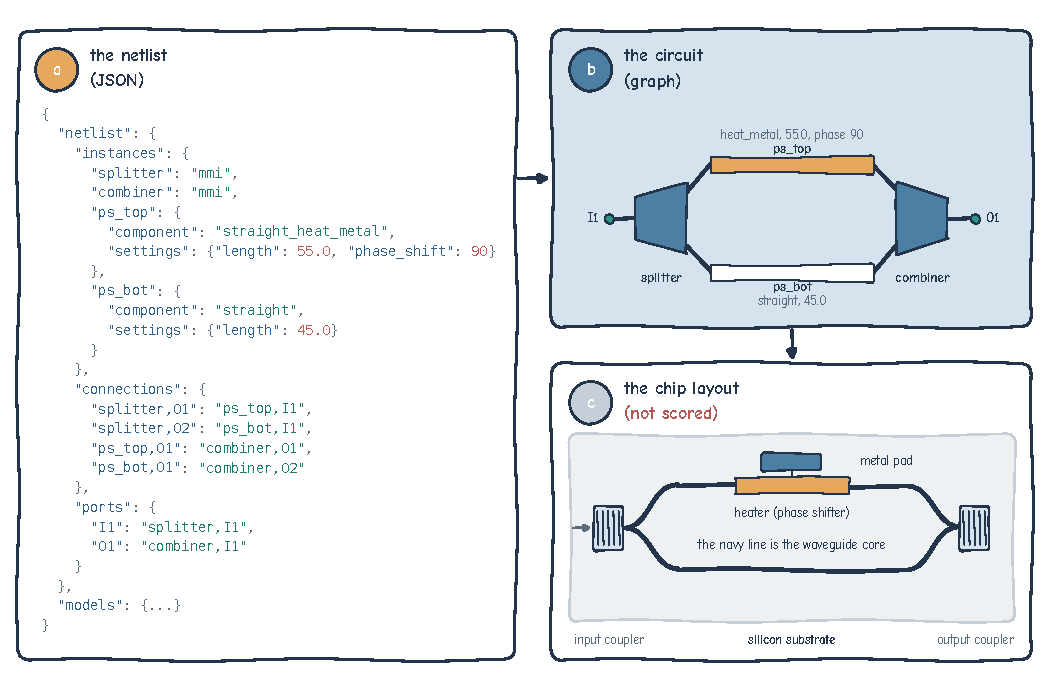
\includegraphics[width=\linewidth]{../paper_figures/fig6_netlist_layout.pdf}
\caption{The object PICBench scores is the JSON netlist, not the mask.
Panel (a) is one Mach--Zehnder: device instances, port bindings, a phase setting, and an arm length.
Panel (b) is the circuit that JSON describes.
Panel (c) is a schematic silicon-photonic layout of the same topology.
A spectrum match does not place or route that layout, and it does not check a PDK cell.
The drawing is an illustration.
It is not one of the 24 expert files, and it was not passed through SAX.}
\label{fig:netlist}
\end{figure}

Aggregate syntax and functional rates leave the causes of failure unresolved. A reply may fail before simulation because it cannot be parsed, or after parsing because its models or ports are invalid. Even a simulable circuit may produce the wrong spectrum. Distinguishing these outcomes is necessary to tell whether fine-tuning improves circuit behavior or only executability.

PhIDO, PICopilot, and Chat-to-Chip sit next to this benchmark and score a different object: GDS validity, design scripts, and metasurface geometry \citep{sharma2025phido,jiang2026picopilot,zhang2025chattoschip}.
On PhIDO queries of at most fifteen components, the strongest models reach end-to-end $\passk{5}$ around 57\%.
A valid mask is a different outcome from a matching $|S|^2$.
PICBench itself reports higher rates once a restriction list is added, or once the simulator error is returned for up to three revisions.
We use the column with neither, Without EF.
There the published functional $\passk{1}$ reaches 8.33\% (Gemini 1.5 Pro) and functional $\passk{5}$ reaches 16.67\% (o1-mini) \citep{wu2025picbench}.

VerilogEval, RTLLM, and AnalogCoder already score electronic netlists by compilation or by tests, with feedback in the AnalogCoder loop \citep{liu2023verilogeval,lu2024rtllm,lai2024analogcoder}.
\citet{hedayati2026levels} show that schema, topology, executability, and component-set agreement come apart: 16 of 150 circuits failed a topological check and still ran in ngspice, one of them a dangling resistor at 5.00~V instead of 2.50~V.
NetlistBench applies a structural IR oracle to 2{,}342 SPICE cases \citep{ma2026netlistbench}.
We extend this distinction to photonic netlist generation by auditing failures at each evaluation stage and testing supervision built from those failures. We compare answer distillation \citep{hinton2015distilling} with direct supervision on the reference JSON, which already specifies the devices, wiring, and parameters. This control tests whether teacher replies provide a measurable benefit beyond the reference circuit itself.

We evaluate Qwen3.5-9B \citep{qwen2026}, DeepSeek-V4-Pro \citep{deepseek2026v4}, Qwen3.6-27B, GLM-5.3, and DeepSeek-V4.1-Flash on all 24 designs, with five samples each. The prompt, temperature, and judge are shared; model size, deployment, and reasoning configuration differ. We then compare two forms of supervision on the same synthetic questions: filtered teacher replies and reference JSON. Both improve executability, but their epoch-8 functional counts remain 4/120 and 0/120.

Per-sample accuracy and design-level coverage diverge: GLM-5.3 posts the highest functional $\passk{1}$ (39.17\%) yet a functional $\passk{5}$ (54.17\%) below Qwen3.6-27B's 70.83\%, whose per-sample rate is lower but whose passing samples spread across more designs (Figure~\ref{fig:pareto}).

\begin{figure}[t]
\centering
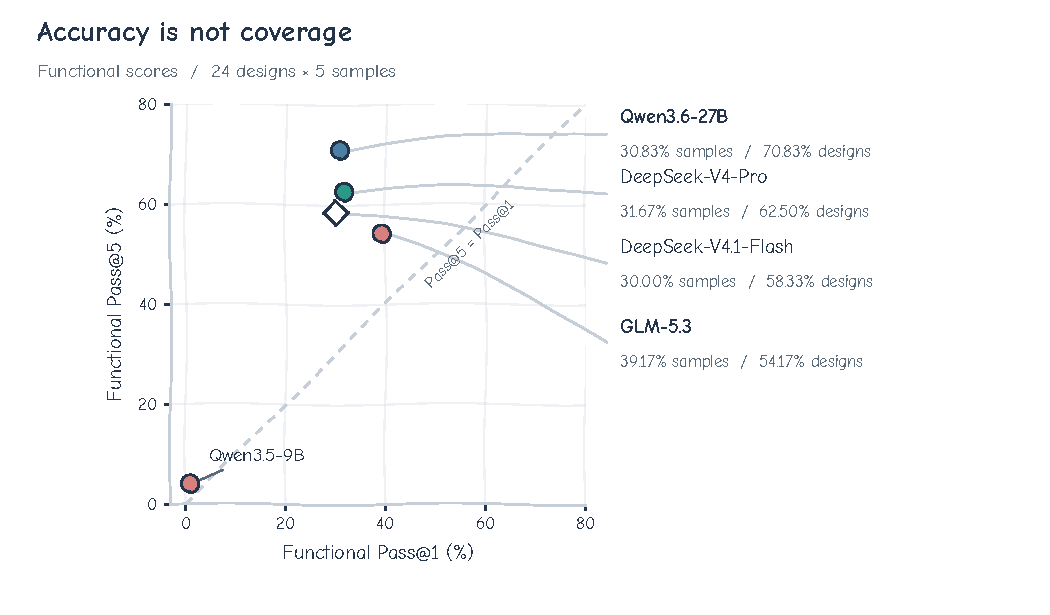
\includegraphics[width=\linewidth]{../paper_figures/fig5_model_pareto.pdf}
\caption{Functional accuracy and design coverage for the five measured models. $\passk{1}$ is the fraction of matching samples; $\passk{5}$ is the fraction of designs with at least one match. GLM-5.3 has the highest sample accuracy but covers fewer designs than Qwen3.6-27B. The axes use equal scales; the dashed line marks equal rates. Model size, deployment, and reasoning configuration differ across runs.}
\label{fig:pareto}
\end{figure}

Our contributions are threefold:
\begin{itemize}
\item A stage-level audit of five models under Without EF, separating extraction and parsing failures, simulator rejection, and spectral mismatch. Among the four API models, only 48.0--56.3\% of simulable netlists match the reference spectrum.
\item A circuit-first generator of 1{,}000 questions targeting observed failure categories, with lexical and structural overlap checks. The categories are informed by test failures, and their manually assigned weights have not been compared with random circuit synthesis.
\item A matched comparison of teacher-answer and reference-JSON supervision on 985 spectrally checked questions. At epoch 8, teacher answers improve functional design coverage over reference JSON but fall below the pre-specified sample-accuracy threshold. Both students perform worse than the base model on NetlistBench, providing no evidence of transfer to SPICE.
\end{itemize}

\begin{figure}[t]
\centering
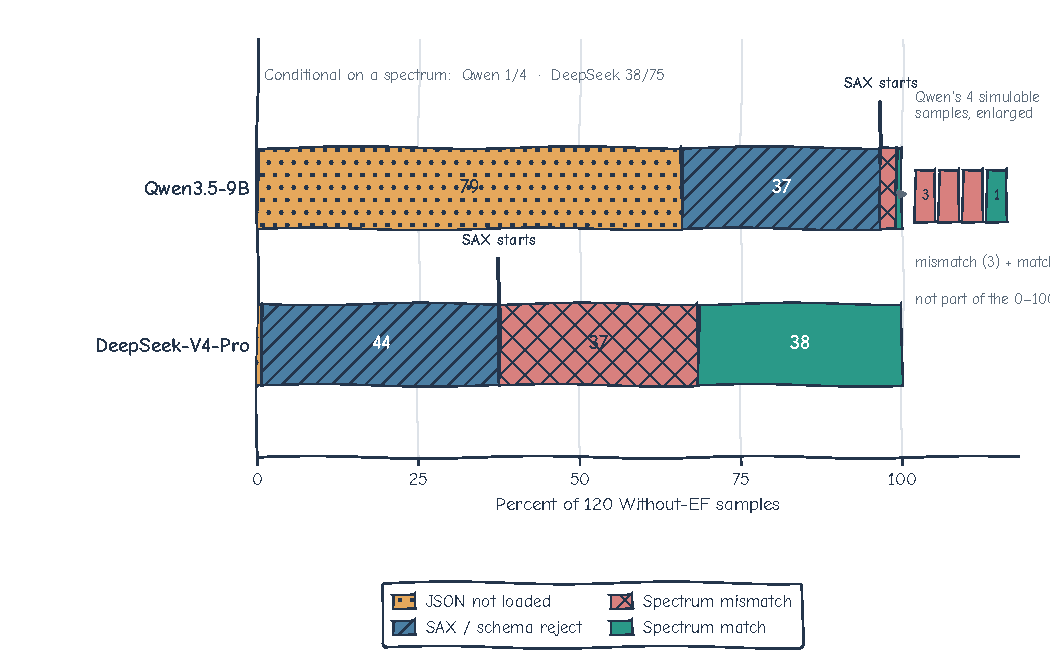
\includegraphics[width=\linewidth]{../paper_figures/fig1_failure_audit.pdf}
\caption{Each bar is 120 Without-EF samples, stacked by the mutually exclusive stage in which the judge rejected or accepted the netlist.
``JSON not loaded'' joins a missing result span (7 for Qwen3.5-9B, 1 for DeepSeek-V4-Pro) to a \texttt{json.loads} rejection (72 and 0).
The navy tick marks where SAX starts: simulable netlists begin to its right.
For Qwen that region is a thin sliver---three spectrum mismatches and one match---so the four cells on the right repeat those samples at equal width, marked enlarged, outside the 0--100 axis.
Syntax pass is the mismatch plus match segments, and functional pass the match segment alone; counts are Table~\ref{tab:loci}.}
\label{fig:twostage}
\end{figure}

\section{Related work}

\paragraph{Photonic language-model generators.}
PICBench is a natural-language-to-netlist benchmark for photonic integrated circuits \citep{wu2025picbench}.
Its 24 problems cover six optical-computing circuits, seven optical-interconnect circuits, nine optical switches, and two fundamental devices that themselves contain connections.
Each problem ships a description, an expert netlist, and the SAX spectrum of that netlist.
Syntax is ``SAX can simulate.''
Function is ``the simulated transmission matches the expert file.''
The original evaluation uses the unbiased $\passk{k}$ estimator of \citet{chen2021codex} with $n=5$ samples per design.
We use that estimator and that judge without changing the rounding or the wavelength grid.
Without restrictions and without feedback, the published syntax $\passk{1}$ ranges from 8.33\% to 16.67\% and functional $\passk{1}$ from 1.67\% to 8.33\%; adding the authors' restriction list, or returning the simulator error for up to three revisions, raises both numbers.
We use the no-restriction, zero-feedback column, labeled Without EF, transcribed in Table~\ref{tab:published}, and we did not rerun the five commercial models.

PhIDO converts a natural-language photonic request into a GDS layout through a multi-agent loop \citep{sharma2025phido}.
Its testbench has 102 descriptions, from single devices to 112-component circuits, and its headline number is structural: whether the generated mask is a valid layout, not whether a compact-model spectrum matches an expert file.
For queries of at most fifteen components, o1, Gemini-2.5-Pro, and Claude Opus 4 reach end-to-end $\passk{5}$ around 57\%.
PICopilot generates design scripts rather than netlists, with retrieval and feedback, and reports that all 48 of its scripting tasks complete \citep{jiang2026picopilot}.
Chat-to-Chip fine-tunes language models to predict spectra and invert arbitrarily shaped metasurfaces \citep{zhang2025chattoschip}.
The output is a geometry token sequence, not a SAX JSON graph, and none of these systems partitions load failures on a nested $|S|^2$ judge or separates a reference-JSON student from a teacher-answer student.

SAX is an $S$-parameter circuit simulator built on JAX \citep{laporte2023sax}.
Given a JSON netlist and a dictionary of device models, it returns the scattering matrix on a wavelength grid.
PICBench builds models for waveguides, couplers, multimode interferometers, Mach--Zehnder stages, microrings, and phase shifters, and it simulates 1{,}000 wavelengths from 1.51 to 1.59~$\mu$m.
A functional match is a property of those curves, inside a fixed compact model, with layout, full-wave electromagnetics, and fabrication outside the judge.

\paragraph{Syntax versus function in electronic netlists.}
The electronic relatives of the task already treat compilation and tests as different events.
VerilogEval and RTLLM score generated RTL by execution rather than by text overlap \citep{liu2023verilogeval,lu2024rtllm}.
AnalogCoder generates PySpice, repairs against simulator feedback, and reports 20 of 24 analog tasks solved \citep{lai2024analogcoder}.
ChipNeMo domain-adapts LLMs for an engineering chatbot, EDA scripts, and bug summaries; it is an adaptation result, not a nested syntax/function partition of a netlist benchmark \citep{liu2023chipnemo}.
\citet{hedayati2026levels} makes the partition explicit for LLM-generated circuits: schema validity, topological validity, backend executability, and component-set agreement are four levels, and they are not nested.
On 150 circuits, 16 were rejected by a topological validator and still executed in ngspice without a warning; a dangling resistor in a divider produced 5.00~V instead of 2.50~V while the simulator stayed silent.
That is the electronic form of a legal-but-wrong netlist.
NetlistBench asks a related question about SPICE rather than photonic JSON \citep{ma2026netlistbench}.
Its oracle compares a canonical intermediate representation over 2{,}342 recognition and edit cases; a SPICE pass rate is not a PICBench $\passk{k}$.
Section~\ref{sec:spice} reports the 9B zero-shot score and both epoch-8 students on that oracle in separate tables, and the 2{,}342 released cases stay out of both training pools.

\paragraph{Answer distillation.}
We fine-tune a student on a stronger model's visible replies, a form of answer distillation \citep{hinton2015distilling}. The target includes the visible analysis and result block; the separate API reasoning trace is excluded from the loss. Our reference-JSON control uses the same questions and training procedure but directly supervises the reference circuit. This comparison isolates the effect of the supervision target within the chosen training procedure, rather than comparing circuit supervision with formatting alone.

\section{Measurement protocol}
\label{sec:protocol}

\subsection{Judge}

For each decoded netlist, PICBench's \texttt{evaluate} returns a verdict string. We retain its official syntax and functional metrics and resolve the evaluation into five mutually exclusive outcomes: extraction failure, JSON parse failure, SAX/schema rejection, simulation-valid spectral mismatch, and spectral match.

Extraction fails when the saved reply has no usable \texttt{\textless result\textgreater} span, so nothing is passed to the judge.
JSON parsing fails when \texttt{json.loads} rejects that span.
A fence, a \texttt{//} comment, an ellipsis, or trailing prose can all land there, and none of them is a SAX result.
Simulation-valid means SAX returns a finite spectrum on
\[
\lambda_i = 1.51 + (1.59-1.51)\frac{i}{999}, \qquad i=0,\ldots,999,
\]
in microns, with $|S_{pq}(\lambda_i)|^2$ recorded for every external input--output pair the candidate declares, and with the same number of curves as the expert file.
PICBench calls every such reply a syntax pass, including replies whose spectrum does not match.
A spectrum match requires those curves, rounded to ten decimal places, to be equal as sets; PICBench calls that a functional pass, and the rounding and set comparison are the benchmark's.
A matching spectrum is a subset of the simulation-valid replies, so the two official rates share samples.

A parsed JSON object can still miss a model name, and a simulation-valid netlist can still disagree with the expert file.

\subsection{\texorpdfstring{Pass@$k$, and a conditional rate}{Pass@k, and a conditional rate}}

Each design is sampled $n=5$ times.
If $c$ of those samples pass a given criterion,
\begin{equation}
\label{eq:passk}
\passk{k}
=
\mathbb{E}_{d}
\left[
1 - \frac{\binom{n-c_d}{k}}{\binom{n}{k}}
\right],
\end{equation}
where the binomial ratio is replaced by $0$ when $n-c_d < k$, the usual unbiased estimator \citep{chen2021codex}.
We report $k=1$ and $k=5$, averaged over the 24 designs that all have five completed samples.
With $n=k=5$, $\passk{5}$ equals the fraction of designs with at least one passing sample, and with equal $n$, $\passk{1}$ equals the number of passing samples divided by 120.
One design moving from $0/5$ to $1/5$ changes $\passk{1}$ by $1/120 = 0.83$ points and $\passk{5}$ by $1/24 = 4.17$ points.
Sample accuracy and design coverage therefore require separate thresholds: ten additional matching samples increase $\passk{1}$ by $10/120$, whereas two newly covered designs increase $\passk{5}$ by $2/24$, even if each contributes only one match. Section~\ref{sec:prereg} specifies a threshold for each metric.
The 120 draws are not treated as independent: five samples share a prompt, and the expectation in \eqref{eq:passk} is over designs.

We also report
\[
\mathbb{P}(\text{function}\mid\text{syntax})
=
\frac{\#\{\text{matching spectra}\}}{\#\{\text{simulable netlists}\}}.
\]
This conditional rate measures spectral correctness among simulation-valid netlists. It complements $\passk{k}$: increasing executability alone need not increase the number of functional matches and may lower the conditional match rate.

\subsection{Prompt and decoding}

The prompt is the one in PICBench's generator for a run with restrictions turned off and with zero feedback iterations.
The system message is \texttt{system\_prompt.txt}: a SAX JSON schema, the built-in device list, and the requirement that the reply contain an analysis followed by a \texttt{\textless result\textgreater} block.
The restrictions file is not concatenated.
One in-context example, the published Mach--Zehnder question and its published answer, precedes the test item.
The user message is the problem text plus the published instruction, which asks for a JSON netlist and, in the same sentence, for advice ``based on the restrictions.''
That sentence survives even though the restriction list is absent, because it is what \texttt{gen\_data.py} sends, and the official client places the whole user message twice, once inside the seeded dialogue and once as the next turn; our calls do the same.

The published one-shot answer connects both waveguides to the same combiner input, which is illegal under the simulator's one-connection-per-port rule.
We leave it in place because it is part of the prompt the Without-EF column used; the example does not make a legal netlist unreachable.

Qwen3.5-9B is the local post-trained checkpoint, loaded in bfloat16.
Thinking is disabled, so the sampled tokens are the visible reply.
Generation uses temperature $1$, top-$p$ $1$, a torch seed equal to the sample index, a limit of 32{,}768 new tokens, and a stop string at \texttt{\textless /result\textgreater}.
DeepSeek-V4-Pro is the API model name \texttt{deepseek-v4-pro}, called on 20 October 2026 at temperature $1$ with a 32{,}768-token completion budget and no stop string.
The API returned a reasoning trace on every call.
Scoring uses the netlist parsed from the string \texttt{reply\_text} stores.
That string is the visible \texttt{content} when \texttt{content} contains \texttt{\textless result\textgreater}, which is true of 118 of the 120 calls.
On the other two calls the visible content has no such tag.
Crossbar $4\times4$ sample 1 has the tag only in \texttt{reasoning\_content}, and the scorer falls back to that trace.
The stored netlist is rejected for the model name \texttt{osu}; it is neither simulation-valid nor a spectrum match, so the fallback leaves both $\passk{k}$ unchanged.
It does move the stage table: under a visible-content-only rule this sample would be a second extraction failure and the model-name rejections would be 7 rather than 8.
U-matrix sample 2 has the tag in neither field.
That is the one extraction failure in Table~\ref{tab:twostage} and Table~\ref{tab:loci}.
Ten reasoning traces contain \texttt{\textless result\textgreater}, but nine of those calls also carry the tag in the visible content, and the visible content is what was scored; the local 9B run has no separate reasoning field, and its judged string is the visible generation.

Both runs cover $24 \times 5 = 120$ samples.
Every DeepSeek call ended with finish reason \texttt{stop}; one Qwen call hit the 32{,}768-token cap.
The shared prompt, temperature, sample count, and judge do not make the runs a controlled comparison of reasoning.
Qwen is a local 9B checkpoint with thinking disabled.
DeepSeek-V4-Pro is an API model that returned a reasoning trace on every call, and we do not have its weight hash or a matched token budget for that trace.

\subsection{Shared protocol}

Relative to Table~III Without EF, we share the problem texts, the system prompt, the in-context example, the double user turn, the absence of \texttt{restrictions.txt}, zero error feedback, $n=5$, and the SAX judge.
Our temperature is $1$ and top-$p$ is $1$ for the local 9B run, the historical default of the chat interface the original code calls. The API request for DeepSeek-V4-Pro sets temperature $1$ and does not set a separate top-$p$.
The original paper does not publish a temperature, a token cap, or a seed, and we did not rerun its five commercial models, so the first five rows of Table~\ref{tab:published} are transcribed from that paper and the last five are our measurements.
Qwen3.6-27B, GLM-5.3, and DeepSeek-V4.1-Flash were evaluated subsequently on the same 24 problems, with the same prompt, temperature $1$, sample count, and SAX judge. Qwen3.6-27B used a 65{,}536-token completion cap. GLM-5.3 used 131{,}072 tokens for 117 calls and 32{,}768 for three; DeepSeek-V4.1-Flash used 32{,}768 tokens for 119 calls and 131{,}072 for one.
The five measured rows still do not hold scale, deployment, or the token budget fixed.
Designs that are short of five samples stay out of every $\passk{k}$ in this paper.

\section{Zero-shot results}
\label{sec:results}

\begin{table}[H]
\caption{Syntax and functional $\passk{k}$ on PICBench, in percent.
The first five rows are transcribed from Table~III of \citet{wu2025picbench}, Without EF, and were not rerun.
The last five rows use the protocol in Section~\ref{sec:protocol}.
Syntax includes functional matches.}
\label{tab:published}
\begin{center}
\begin{small}
\begin{tabular}{lrrrr}
\toprule
Model & \multicolumn{2}{c}{$\passk{1}$} & \multicolumn{2}{c}{$\passk{5}$} \\
\cmidrule(lr){2-3}\cmidrule(lr){4-5}
 & Syn. & Func. & Syn. & Func. \\
\midrule
GPT-4 & 16.67 & 6.67 & 41.67 & 12.50 \\
o1-mini & 8.33 & 4.17 & 29.17 & 16.67 \\
GPT-4o & 14.17 & 4.17 & 37.50 & 4.17 \\
Claude 3.5 Sonnet & 13.33 & 1.67 & 20.83 & 8.33 \\
Gemini 1.5 Pro & 9.17 & 8.33 & 16.67 & 12.50 \\
\midrule
Qwen3.5-9B & 3.33 & 0.83 & 16.67 & 4.17 \\
DeepSeek-V4-Pro & 62.50 & 31.67 & 95.83 & 62.50 \\
Qwen3.6-27B & 63.33 & 30.83 & 91.67 & 70.83 \\
GLM-5.3 & 81.67 & 39.17 & 100.00 & 54.17 \\
DeepSeek-V4.1-Flash & 53.33 & 30.00 & 91.67 & 58.33 \\
\bottomrule
\end{tabular}
\end{small}
\end{center}
\end{table}

Table~\ref{tab:published} is the main measurement.
Qwen3.5-9B produces 4 simulable netlists and 1 matching spectrum in 120 draws.
Those four draws sit on four designs, one each, so the syntax $\passk{5}$ is $4/24 = 16.67\%$ and the functional $\passk{5}$ is $1/24 = 4.17\%$.
The matching spectrum is one sample of the QPSK modulator.
The other three simulable replies, on the direct modulator, the Mach--Zehnder modulator, and the nonlinear-sign gate, miss the expert spectrum.
The remaining 20 designs are $0/5$ on both criteria.
No optical switch is among the four simulable replies.

DeepSeek-V4-Pro produces 75 simulable netlists and 38 matching spectra.
Syntax $\passk{5}$ is $23/24$: the WDM demultiplexer is the only design with no simulable sample, and all five of its failures are port errors.
Functional $\passk{5}$ is $15/24$.
The nine designs with no functional sample are the $8 \times 8$ Clements, Reck, crossbar, and Spanke--Benes meshes, the phase-shifter MZI, the nonlinear-sign gate, the QPSK modulator, and both WDM circuits.
Direct modulation and the Mach--Zehnder modulator are $5/5$ functional.
The phase-shifter MZI is $5/5$ syntax and $0/5$ functional: the model can emit a netlist the simulator accepts, and the spectrum is still wrong on every draw.
Figure~\ref{fig:syntax-vs-function} shows the same split across all five measured models.

\begin{figure}[t]
\centering
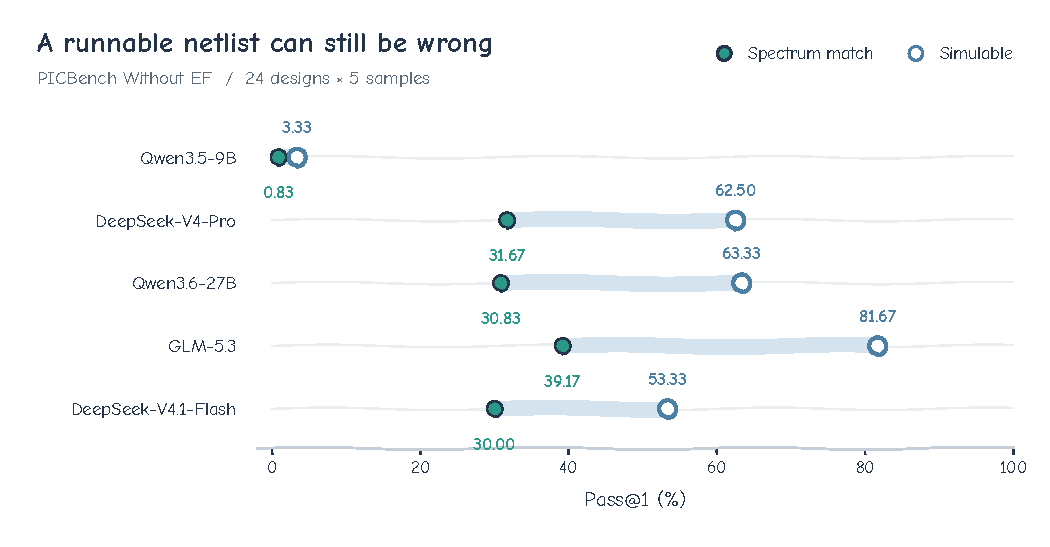
\includegraphics[width=\linewidth]{../paper_figures/fig4_syntax_function_gap.pdf}
\caption{Syntax and functional $\passk{1}$ for the five measured models. Open circles mark simulation-valid samples; filled circles mark spectrum matches. Each connecting segment is the rate of simulable but nonmatching samples. The four API models span 53.33--81.67\% on syntax but only 30.00--39.17\% on function. Model size, deployment, and reasoning configuration differ across runs.}
\label{fig:syntax-vs-function}
\end{figure}

\begin{table}[H]
\caption{Outcomes on the string the Without-EF judge actually scored.
Extraction failure means that scored string had no usable result span.
For DeepSeek, 118 visible contents contain the tag; one further netlist was read from the reasoning trace and then rejected for a model name, so the extraction-failure count stays 1.
JSON parse failure means \texttt{json.loads} rejected that span.
The next row is a parsed object that SAX or the model dictionary rejected.
$\mathbb{P}(\text{function}\mid\text{syntax})$ is matching spectra over simulable netlists.}
\label{tab:twostage}
\begin{center}
\begin{small}
\begin{tabular}{lrr}
\toprule
Quantity & Qwen3.5-9B & DeepSeek-V4-Pro \\
\midrule
Simulable / 120 & 4 & 75 \\
Matching / 120 & 1 & 38 \\
$\mathbb{P}(\text{function}\mid\text{syntax})$ & $1/4 = 25\%$ & $38/75 = 50.7\%$ \\
Extraction failure / 120 & 7 & 1 \\
JSON parse failure / 120 & 72 & 0 \\
Parsed, SAX or schema rejects / 120 & 37 & 44 \\
\bottomrule
\end{tabular}
\end{small}
\end{center}
\end{table}

The 9B model almost never reaches the simulator; DeepSeek-V4-Pro almost always does, and it is right on 38 of 75 simulable netlists.
Moving mass from the unloadable rows into the simulable row would raise syntax $\passk{1}$, not functional $\passk{1}$, and Reference-JSON epoch 8 does exactly that: 31 simulable netlists against 4 at zero shot, with 0 spectrum matches.

The models succeed on different subsets of designs, so aggregate rates do not establish item-wise dominance. DeepSeek-V4-Pro's functional $\passk{1}$ exceeds the transcribed Without-EF results, although differences in model deployment and undocumented historical decoding settings limit direct comparisons.

\begin{table}[H]
\caption{Simulable / matching samples by PICBench family, out of the family total.
Totals are 30 computing, 35 interconnect, 45 switch, and 10 device samples (six, seven, nine, and two designs, five each).
DS-V4-Pro is DeepSeek-V4-Pro; V4.1-Flash is DeepSeek-V4.1-Flash.}
\label{tab:family}
\begin{center}
\begin{small}
\begin{tabular}{lccccc}
\toprule
Family & Qwen3.5-9B & DS-V4-Pro & Qwen3.6-27B & GLM-5.3 & V4.1-Flash \\
\midrule
Computing & 1/0 & 15/6 & 19/3 & 27/1 & 13/3 \\
Interconnect & 2/1 & 19/8 & 25/14 & 21/9 & 15/13 \\
Switch & 0/0 & 31/19 & 26/17 & 41/33 & 29/15 \\
Devices & 1/0 & 10/5 & 6/3 & 9/4 & 7/5 \\
\bottomrule
\end{tabular}
\end{small}
\end{center}
\end{table}

Table~\ref{tab:family} breaks the same 120 samples by PICBench family.
Qwen's simulable replies are confined to interconnect and device problems plus the nonlinear-sign gate; no switch contributes.
DeepSeek simulates every device sample and matches half of them, while GLM's functional mass concentrates on switches (33/45) and nearly vanishes on computing (1/30).

\begin{table}[H]
\caption{DeepSeek-V4-Pro on the six architectures that PICBench poses at both $4 \times 4$ and $8 \times 8$.
Each cell is the number of simulable samples and, after the slash, the number whose spectrum matches, out of five.}
\label{tab:width}
\begin{center}
\begin{small}
\begin{tabular}{lcc}
\toprule
Architecture & $4 \times 4$ & $8 \times 8$ \\
\midrule
Clements & 4/2 & 2/0 \\
Reck & 2/1 & 2/0 \\
Crossbar & 3/1 & 3/0 \\
Spanke & 3/2 & 4/3 \\
Benes & 4/4 & 2/2 \\
Spanke--Benes & 4/4 & 3/0 \\
\midrule
All six & 20/14 & 16/5 \\
\bottomrule
\end{tabular}
\end{small}
\end{center}
\end{table}

Width is informative for the model that can already emit meshes: across the six paired architectures, DeepSeek's functional count falls from 14/30 at width 4 to 5/30 at width 8, with Spanke the one exception.
Qwen is $0/5$ on all twelve items.
The drop is why the training generator in Section~\ref{sec:lociq} never emits width $4$ or $8$, and per-design counts are in Appendix~\ref{app:perdesign}.

\subsection{Three further API runs}
\label{sec:api}

Qwen3.6-27B produces 76 simulable netlists and 37 matching spectra (syntax $\passk{5}$ 22/24, functional $\passk{5}$ 17/24, conditional match rate 48.7\%).
GLM-5.3 produces 98 simulable netlists and 47 matching spectra (syntax $\passk{5}$ 24/24, functional $\passk{5}$ 13/24, conditional match rate 48.0\%), and every design has at least one simulable sample.
GLM's functional $\passk{1}$ is the highest of the five rows and its functional $\passk{5}$ is below Qwen3.6-27B's, because more matching samples are concentrated on fewer designs (Figure~\ref{fig:pareto}).
The phase-shifter MZI is again $5/5$ syntax and $0/5$ function for GLM, the same split DeepSeek shows on that item.
Qwen3.6-27B matches the WDM demultiplexer on $4/5$ draws, a design DeepSeek-V4-Pro never simulates, and matches the U-matrix block on $0/5$, a design DeepSeek-V4-Pro matches on $3/5$.
DeepSeek-V4.1-Flash produces 64 simulable netlists and 36 matching spectra (syntax $\passk{5}$ 22/24, functional $\passk{5}$ 14/24, conditional match rate 56.3\%), and its failure stage differs from DeepSeek-V4-Pro's: 54 of 120 verdicts are port errors, against 24.

\begin{table}[H]
\caption{Verdict strings for the three later API runs.
The per-design \texttt{syntax} integer in the score files counts spectrum mismatches only, so this table is taken from the verdict strings.
``Missing models'' is the schema string inside an \texttt{other syntax} verdict, kept separate from the \texttt{wrong model} prefix.}
\label{tab:api}
\begin{center}
\begin{small}
\begin{tabular}{lrrr}
\toprule
Quantity & Qwen3.6-27B & GLM-5.3 & Flash \\
\midrule
Simulable / 120 & 76 & 98 & 64 \\
Matching / 120 & 37 & 47 & 36 \\
$\mathbb{P}(\text{function}\mid\text{syntax})$ & $37/76$ & $47/98$ & $36/64$ \\
Wrong-model prefix / 120 & 11 & 1 & 0 \\
Wrong ports / 120 & 11 & 11 & 54 \\
Missing models / 120 & 4 & 10 & 2 \\
Other SAX or schema rejection / 120 & 18 & 0 & 0 \\
Extraction or JSON failure / 120 & 0 & 0 & 0 \\
\bottomrule
\end{tabular}
\end{small}
\end{center}
\end{table}

Table~\ref{tab:api} uses the official verdict strings, whereas Table~\ref{tab:twostage} additionally re-audits extraction and parsing. No scored file in these three runs fails either step. Among simulation-valid samples, 39, 51, and 28, respectively, fail spectral comparison.

\section{Where the 9B replies fail}
\label{sec:loci}

The 120 Qwen verdicts separate replies rejected before simulation from legal netlists with wrong spectra. Table~\ref{tab:loci} labels the exact string passed to \texttt{evaluate}; it supersedes an earlier whole-reply heuristic that counted 97 surface-format failures.

\begin{table}[H]
\caption{Stage of the stored netlist, the string the Without-EF judge scored.
JSON parse reasons for Qwen, which can overlap inside one string, are ellipsis 44, trailing text 15, \texttt{//} 5, a fence that survived extraction 4, and other parse errors 4.
``SAX or schema rejects'' splits, for Qwen / DeepSeek, into SAX runtime 25/12, model name 9/8, and ports 3/24.}
\label{tab:loci}
\begin{center}
\begin{small}
\begin{tabular}{lrr}
\toprule
Stage of the stored netlist & Qwen3.5-9B & DeepSeek-V4-Pro \\
\midrule
No usable result span & 7 & 1 \\
\texttt{json.loads} rejects the span & 72 & 0 \\
Parsed; SAX or the schema rejects it & 37 & 44 \\
Simulation-valid; spectrum differs & 3 & 37 \\
Spectrum matches the expert file & 1 & 38 \\
\midrule
Total & 120 & 120 \\
\bottomrule
\end{tabular}
\end{small}
\end{center}
\end{table}

Seventy-nine Qwen replies never yield an object the judge can load, 44 of the 72 parse failures because an ellipsis stands where repetitive entries should be.
The length cap does not explain the table: the single capped reply is one sample of \texttt{WDM\_mux}, already $0/5$ on the four uncapped samples.

The failures cluster on larger circuits: 45 of 60 Qwen samples on the twelve width-$4$ and width-$8$ meshes fail extraction or parsing; the same is true for 36 of 45 switch samples. The training pool does not test whether its shorter circuits address this limitation.

DeepSeek contributes one extraction failure and zero parse failures; of its 75 simulable netlists, 38 match the expert spectrum and 37 do not, so a simulation-valid netlist is still not a spectrum match.
The dominant error that blocks simulation is the port map (24 replies), followed by other SAX errors (12) and undefined model names (8).
On PICBench's two device designs, DeepSeek is $10/10$ simulation-valid but only $5/10$ functional. All five mismatches occur on the phase-shifter MZI.

\subsection{Format repair}
\label{sec:repair}

Before any fine-tune, a deterministic cleanup asks how much of the load failure is post-processing.
The cleanup does not read the expert netlist and does not fill in an ellipsis; it strips fences, drops lines that are only \texttt{//} comments, and keeps the first JSON object.
The cleaned strings are a modified protocol, kept out of Table~\ref{tab:published}.

On Qwen, the cleanup moves the 120 replies to 6 simulation-valid netlists and 2 spectrum matches (functional $\passk{1}$ 1.67\%, $\passk{5}$ 8.33\%).
After cleanup, 40 originally unparseable replies reach SAX or schema validation but are rejected, and 17 still contain no complete object. Recovering a JSON object rarely recovers the intended circuit.

On DeepSeek, the same cleanup recovers one additional spectrum match; functional $\passk{1}$ moves from 31.67\% to 32.50\%, $\passk{5}$ stays $15/24$.

The distinction also follows directly from the stage counts: converting all 79 extraction or parse failures into simulable but incorrect netlists would raise Qwen's syntax count from 4 to 83 without adding a single functional match. This is a hypothetical bound on executability, not an estimate of what repair or training would achieve.

\section{Failure-locus questions}
\label{sec:lociq}

We construct synthetic circuits separately from the 24 evaluation problems, using categories informed by the 9B model's test failures. We call this procedure \emph{failure-locus verbalization} (Figure~\ref{fig:verbalization}). Its six families---ellipsis, comment, wrong model, ports, function, and graft---target specific generation errors rather than PICBench's application categories. Graph construction precedes prose generation, and widths $4$ and $8$ are excluded. Table~\ref{tab:construct} summarizes the procedure.

\begin{table}[H]
\caption{Failure-locus verbalization.
The unit of sampling is a legal SAX graph.
Generation does not read the 24 expert netlists.
A later fingerprint screen does.
The 9B text-heuristic labels choose the families; the weights are fixed and were not refit.}
\label{tab:construct}
\begin{center}
\begin{small}
\begin{tabular}{lll}
\toprule
Move & What is sampled & What is left out \\
\midrule
Index & 9B text-heuristic labels & PICBench device families \\
Order & Graph $\to$ SAX $\to$ prose; JSON held out & Prose first; JSON in the prompt \\
Isolate & Contrast sets; width $\in \{2,3,5,6\}$ & Mix id with topology; width $4$ or $8$ \\
\bottomrule
\end{tabular}
\end{small}
\end{center}
\end{table}

The generator, with seed \texttt{20261020}, is the following procedure.
The input is the PICBench device library and the earlier text-heuristic labels, not the re-audit in Table~\ref{tab:loci}.
The family weights were not refit after that audit.
The output is a question whose prompt is prose and whose \texttt{reference} field is JSON.
\begin{enumerate}
\item Draw a family with the fixed weights in Table~\ref{tab:train}: ellipsis 280, comment 160, wrong model 280, ports 80, functional 120, graft 80.
\item Sample one free variable inside that family.
Widths are uniform in $\{2,3,5,6\}$.
A wrong-model item copies the wiring of its contrast partner and changes one SAX identifier.
\item Reject the draw if a port is used twice, an external binding is dangling, the external width is $4$ or $8$, an eight-word shingle hits a test problem or the in-context example, or the text names 8-QAM, 64-QAM, or the test WDM wavelengths.
\item Call SAX on eight wavelengths in $[1.51, 1.59]$.
Keep the draw only when every transmission is finite.
The eight-wavelength check is separate from the 1{,}000-point equality test.
\item Write the prose from the graph, store the JSON as \texttt{reference}, and leave the restrictions file off.
\end{enumerate}
No ablation against a random draw of the same size has been run, so the procedure does not say whether failure-locus sampling beats ordinary synthetic circuits; that comparison would need the same question count, student, budget, and Without-EF judge.
The reference-JSON control in Section~\ref{sec:prereg} is a different comparison---its epoch-8 score is 31 simulable netlists and 0 matches, and it is not a random-synthesis ablation.

The weights in Table~\ref{tab:train} are a hand-set allocation, not fitted to the text-heuristic frequencies or to Table~\ref{tab:loci}.
Ellipsis and wrong-model each receive 280 items, matching the two skills the 9B run lacked: finishing a long repetitive object and keeping a SAX identifier with the wiring fixed.
Comment items (160) force distinct numeric settings into a heater chain, while port items are only 80, although DeepSeek's dominant simulation block is the port map (24 of 120).
No frequency-refit ablation has been run.

The prompt also receives none of the format bans that PICBench derived from its own test-time errors; those bans are the restriction list, and using them here would leave the Without-EF protocol.
The same 1{,}000 items are the question pool for both arms in Section~\ref{sec:prereg}, and copying \texttt{reference} supervises the gold circuit, including the schema.

\begin{figure}[t]
\centering
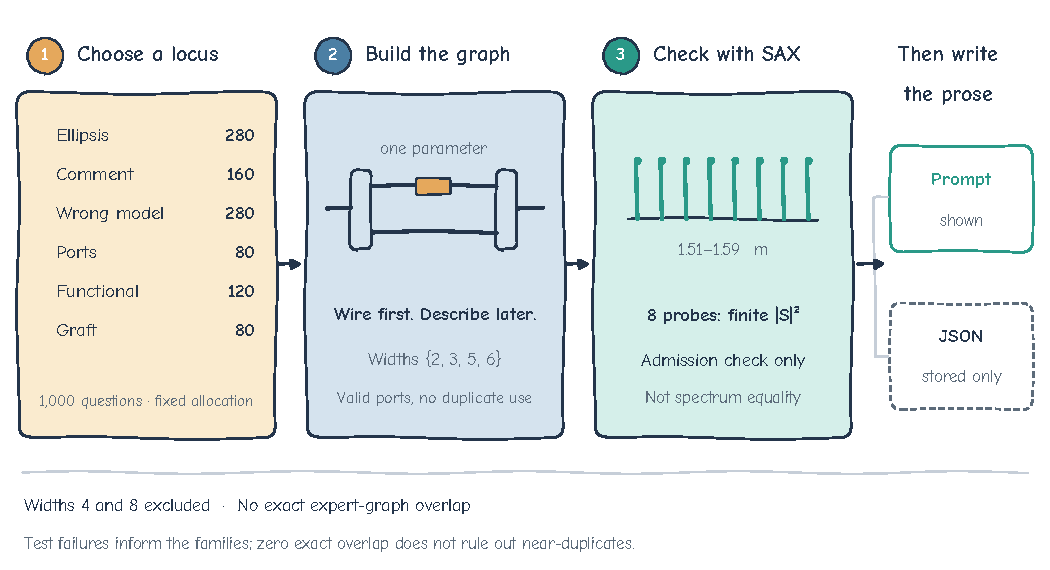
\includegraphics[width=\linewidth]{../paper_figures/fig2_failure_verbalization.pdf}
\caption{Circuit-first question generation. The six family counts are manually allocated from an earlier failure heuristic, not fitted to Table~\ref{tab:loci}. A schematic circuit illustrates graph construction; eight wavelength probes check finiteness, not spectral equality. The prose enters the prompt; the reference JSON is stored separately. Widths $4$ and $8$ are excluded. No reference exactly matches an expert graph fingerprint, but near-duplicates and test-informed family selection remain possible.}
\label{fig:verbalization}
\end{figure}

\subsection{One contrast set}
\label{sec:example}

Questions \texttt{q0441}, \texttt{q0548}, and \texttt{q0555} are one wrong-model group, \texttt{sand-17-81}.
The records are in the question file shipped with the manuscript.
Each prompt asks for the same path: a straight waveguide of length 17, a single-drive or interferometric core, and a heated tail with length 16 and phase 81.
The three references differ only in the core identifier, \texttt{mzm}, \texttt{mzi}, or \texttt{mzm\_dual}, and in the matching \texttt{models} entry; Appendix~\ref{app:example} prints the \texttt{q0441} prompt and its reference.
The prompt names the SAX models in prose, and the JSON is not in the prompt, because a model that can see the reference can satisfy the item by copying it.
The graph is built and checked before that prose is written, and the check that admitted the item is a finite $|S|^2$ on eight wavelengths; the teacher filter, when it is applied, uses the 1{,}000-point equality test against this reference.
Those are different predicates.

\subsection{From a label to a circuit}

The generator draws a legal instance graph, checks that every external port binds to a real device port and that no port is used twice, and calls SAX.
The draw is kept when every transmission on eight wavelengths in $[1.51, 1.59]$ is finite, and the prose description is then written from the same structure.
The random seed is \texttt{20261020}, and all 1{,}000 references passed the finite-spectrum check.

The earlier heuristic categories guide the following circuit families; their allocation was fixed before the stage re-audit in Table~\ref{tab:loci}:
\begin{itemize}
\item Ellipsis questions are parallel chains of identical blocks, width $2$, $3$, $5$, or $6$, so a correct JSON is long and repetitive; the test-mesh widths $4$ and $8$ never appear.
\item Comment questions are chains of heaters in which every length and every phase differs, so the numbers have to live in settings rather than in a copied block.
\item Wrong-model questions are contrast sets that keep the wiring and swap the SAX identifier the 9B run confused, among \texttt{mzi}, \texttt{mzm}, \texttt{mzm\_dual}, \texttt{straight}, \texttt{straight\_heat\_metal}, \texttt{coupler}, \texttt{mzi\_2x2}, \texttt{mzi\_ps}, and \texttt{OSU}; a student that copies a dialect without reading the identifier fails the contrast.
\item Port questions state the external binding in the prompt, including a microring whose three outputs are all exported.
\item Functional questions move one parameter away from the modulator and nonlinear-sign items that reached SAX in the 9B run, and they exclude the test parameter signatures.
\item Graft questions wire two of those fragments in an order the 24 test items do not use: an interferometer into a microring, or one arm of a switch into a modulator.
\end{itemize}
Table~\ref{tab:train} gives the counts, and template counts inside the loci are in Appendix~\ref{app:questions}.

\begin{table}[H]
\caption{The 1{,}000 training questions.
Counts are from the generator manifest.
None of these items is a PICBench test problem.}
\label{tab:train}
\begin{center}
\begin{small}
\begin{tabular}{lrl}
\toprule
Locus & Count & What the prose specifies \\
\midrule
Ellipsis & 280 & Parallel identical chains, width $\in \{2,3,5,6\}$ \\
Comment & 160 & Heater chain, distinct length and phase \\
Wrong model & 280 & Fixed wiring, SAX name is the variable \\
Wrong ports & 80 & External bindings, including every ring port \\
Functional & 120 & One-parameter move off a reached test item \\
Graft & 80 & Interferometer-then-ring, or switch-then-modulator \\
\midrule
Total & 1000 & \\
\bottomrule
\end{tabular}
\end{small}
\end{center}
\end{table}

These families target different requirements: parallel bundles require complete repetitive structures, while contrast sets require the correct SAX identifier even when port names are unchanged. Both supervision arms receive these same circuits; their comparison concerns the training target, not the choice of synthetic questions.

\subsection{What the prompt already contains}
\label{sec:exposure}

Although reference JSON is hidden, every synthetic prompt names its SAX models and includes an explicit \texttt{instance,port} binding. Of the 1{,}000 prompts, 960 use the phrase ``SAX model''; none of the 24 PICBench descriptions does. The teacher filter therefore measures transcription of an explicitly specified circuit, a narrower task than design from a functional specification. Its acceptance rate cannot be read as a PICBench score.

Table~\ref{tab:size} compares the generated graphs with the 24 expert netlists.
Ellipsis items are the long ones---the median bundle has 30 instances and 24 connections, the largest 60 and 54---while the other five families stay near three to seven instances.
The expert files have a median of 7 instances and 8 connections and a maximum of 112 and 160, on the $8\times8$ meshes.
Widths $2$, $3$, $5$, and $6$ are the widths the generator emits, and only the 280 ellipsis items carry a width; widths $4$ and $8$ are both the test mesh sizes and the scale at which DeepSeek's functional count already falls, in Table~\ref{tab:width}.
Holding those widths out avoids copying a test mesh size, but it does not make the training graphs a disjoint circuit family: the 1{,}000 references collapse to 87 structural fingerprints, every fingerprint occurs at least twice, one occurs 73 times, and the settings signatures are far less repetitive, 968 of them distinct.
Repeated topology with varying numbers is what the ellipsis and comment families are built to do, and it is not a broad sample of PICBench meshes; Section~\ref{sec:decontam} records one component-multiset collision with a test expert.

\begin{table}[H]
\caption{Size of the 1{,}000 generated references and the 24 PICBench expert netlists.
Each cell is the median, with the maximum in parentheses.
Only ellipsis items have a width, in $\{2,3,5,6\}$.
The two graft templates are balanced, 40 items each, so the graft row lists both sizes rather than their midpoint.}
\label{tab:size}
\begin{center}
\begin{small}
\begin{tabular}{lrrr}
\toprule
Set & $n$ & Instances & Connections \\
\midrule
Ellipsis & 280 & 30 (60) & 24 (54) \\
Comment & 160 & 5 (7) & 4 (6) \\
Wrong model & 280 & 3 (3) & 2 (2) \\
Ports & 80 & 3 (3) & 2 (2) \\
Functional & 120 & 5 (7) & 5 (6) \\
Graft & 80 & 3 or 6 & 2 or 6 \\
\midrule
PICBench experts & 24 & 7 (112) & 8 (160) \\
\bottomrule
\end{tabular}
\end{small}
\end{center}
\end{table}

\subsection{Decontamination}
\label{sec:decontam}

Decontamination is lexical and structural: an eight-word shingle shared with any of the 24 problem texts, or with the in-context example, rejects the item.
After generation, the longest shared word sequence has length five and occurs on 40 questions, the generic phrase ``one input and one output''; the other 960 share no five-word sequence, and no question contains an eight-word copy of a test problem.
The strings for 8-QAM and 64-QAM are rejected, and so is the test WDM wavelength tuple; mesh widths $4$ and $8$ are rejected by the port check, and the generator's width histogram on the items that carry a width is $\{2: 59,\ 3: 76,\ 5: 70,\ 6: 75\}$.
Neither the expert netlists nor teacher replies to the 24 test prompts are used as training targets. Generation does, however, use the 9B failure labels on those prompts to choose circuit families. PICBench therefore serves as a test-informed evaluation rather than an untouched holdout. The generator does not read expert JSON; a subsequent audit reads the 24 expert netlists solely to compare their fingerprints with the generated references.
Each fingerprint is the multiset of SAX model ids, the multiset of directed port edges after instance names are replaced by (model, local index), and the external port roles.
None of the 1{,}000 training references shares a fingerprint with any of the 24 expert files, so the kept graphs are not those files; that does not make the sampler independent of the test labels, and it does not rule out a near-duplicate.
Twenty functional items, all of template \texttt{coupler\_phase\_line}, share the nonlinear-sign expert's SAX-model multiset---three \texttt{coupler} devices and one \texttt{straight\_heat\_metal}.
Those items have five connections and the expert has four, so the edge fingerprint differs, and the other 980 items share no component multiset with any expert.
Thus the audit finds no exact fingerprint match, but it does identify shared component sets and does not establish independence from the test set. The teacher filter subsequently evaluates all references on the full 1{,}000-point grid. All 1{,}000 produce finite spectra, with no reference-build errors recorded.

\section{Teacher filter}
\label{sec:teacher}

The teacher rollout uses the same prompt as Section~\ref{sec:protocol}, with model name \texttt{glm-5.3}, temperature $0$, one completion per question, and a completion budget of 131{,}072 tokens. A trace is eligible for supervised fine-tuning when the visible content contains \texttt{\textless result\textgreater} and the enclosed JSON parses as an object with both a \texttt{netlist} and a \texttt{models} field; that visible content is the training target, and the reasoning trace is stored but never the target.

Before training, each teacher netlist is compared with its generated reference using the evaluation transmission test: a 1{,}000-point grid, ten-decimal rounding, and set equality of $|S|^2$ curves. Replies that fail this comparison are excluded.
The filter is the same judge as Table~\ref{tab:published}, pointed at the generated references rather than at the 24 expert files.
Run on every reply, it keeps 901 matches as stored, 84 that build only after the missing built-in SAX name is added to \texttt{models} as an identity entry, and drops 15 mismatches (985 kept).
No finished reply fails to parse, and ``match after the name repair'' means SAX rejected the stored file and the same netlist matched once the missing name was added; only these repaired objects are written as the training target.
Table~\ref{tab:teacherlocus} breaks the count down by locus.

\begin{table}[H]
\caption{Teacher filter by the locus of the generated question.
Kept is the sum of the first two columns.
Functional questions were drawn 120 times and graft questions 80 times; the other loci were kept in full.}
\label{tab:teacherlocus}
\begin{center}
\begin{small}
\begin{tabular}{lrrrr}
\toprule
Locus & As stored & Name repair & Dropped & Kept \\
\midrule
Ellipsis & 225 & 55 & 0 & 280 \\
Comment & 160 & 0 & 0 & 160 \\
Wrong model & 252 & 28 & 0 & 280 \\
Ports & 80 & 0 & 0 & 80 \\
Functional & 110 & 0 & 10 & 110 \\
Graft & 74 & 1 & 5 & 75 \\
\midrule
Total & 901 & 84 & 15 & 985 \\
\bottomrule
\end{tabular}
\end{small}
\end{center}
\end{table}

The 84 repairs add missing built-in names to \texttt{models} while the graph, the settings, and the ports stay as the teacher wrote them.
Seventy-six add only \texttt{straight\_heat\_metal}, seven add only \texttt{straight}, and one adds the five names \texttt{mmi1x2}, \texttt{straight}, \texttt{straight\_heat\_metal}, \texttt{coupler}, and \texttt{mrr}.
In each case the addition is exactly the built-in name missing from \texttt{models}, and the repaired object, not the raw file, is written as the training target.
The 90.1\% raw match rate is a rate on these 1{,}000 questions, not a prediction of PICBench performance.

\section{Distillation against reference supervision}
\label{sec:prereg}

Table~\ref{tab:prereg} and Figure~\ref{fig:prereg} compare the base model with two students on the original 24 problems. Both students use the same 985 filtered questions. Reference-JSON SFT targets the reference object enclosed in result tags; Teacher-Answer SFT targets the filtered visible reply, including its analysis and result block, but excludes the separate API reasoning trace. Both targets specify a complete circuit, so Reference-JSON is a circuit-supervision control. No format-only control was run. The decision thresholds below were specified before either trained checkpoint was evaluated on PICBench.

\begin{figure}[t]
\centering
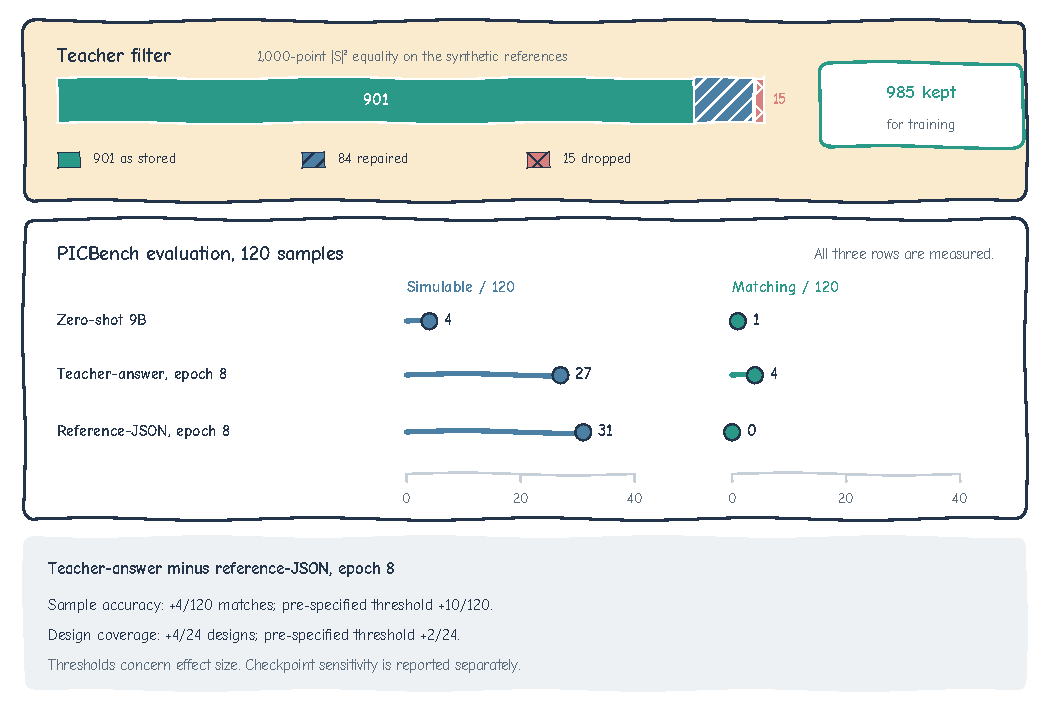
\includegraphics[width=\linewidth]{../paper_figures/fig3_teacher_sft.pdf}
\caption{Teacher filtering and epoch-8 student evaluation. Of 1{,}000 teacher replies, 901 match the synthetic reference as stored, 84 match after a model-dictionary repair, and 15 are dropped. Both students train on the 985 retained questions. Points show counts out of 120 on a common 0--40 scale. Teacher-Answer yields fewer simulable samples than Reference-JSON (27 versus 31), but more spectral matches (4 versus 0). Its advantage meets the pre-specified design-coverage threshold and falls below the sample-accuracy threshold.}
\label{fig:prereg}
\end{figure}

We specified two alternative criteria for a practically relevant advantage of teacher answers over reference JSON: at least $10/120$ additional functional matches ($8.33$ percentage points of $\passk{1}$), or at least $2/24$ additional covered designs on functional $\passk{5}$. These are effect-size thresholds, not significance tests. We report each criterion separately because sample accuracy and design coverage can differ.
A paired resample draws the 24 designs with replacement, 10{,}000 times, seed 20261021, and gives both students the same index on each draw.
The observed gaps are $4/120$ matches and $4/24$ designs; their 2.5--97.5 percentile intervals are $1/120$--$8/120$ and $1/24$--$8/24$, respectively.
The file is \path{logs/picbench/paired_student_bootstrap.json}.
The point estimate meets the design-coverage criterion but not the sample-accuracy criterion. The intervals are descriptive and leave substantial uncertainty about the magnitude of the coverage benefit. Section~\ref{sec:limits} reports corresponding bootstrap intervals for the zero-shot rates. Even a larger advantage would not establish acquisition of general photonic design skills: the training prompts explicitly specify their circuits, and the evaluation contains only 24 test-informed designs.

Teacher-Answer SFT was started from the local post-trained Qwen3.5-9B checkpoint on the 985 kept visible replies.
The update is full-parameter, on four A100-80GB GPUs, ZeRO-3, maximum length 5{,}583, per-device batch size 1, gradient accumulation 2, and a constant learning rate of $5\times10^{-6}$.
Each stage is one epoch of 123 steps; epoch 1 uses warmup ratio 0.05 and seed 42, and later epochs use warmup 0 and seed $41+t$ at epoch $t$.
The launcher keeps a stage when its last-40-step mean loss is at most 98\% of the previous stage's and stops otherwise, up to eight epochs.
The kept target is the visible reply, including the analysis and the \texttt{\textless result\textgreater} block, in the chat template that embeds the duplicated user turn.
The Reference-JSON arm uses that same wrapper, the same 2\% rule, and as its target the question's \texttt{reference} object inside \texttt{\textless result\textgreater}, with no teacher analysis.
The longest row measures 4{,}479 tokens, so \texttt{max\_length} stays 5{,}583.
Its last-40-step means are 0.00577428, 0.00000025, and then 0.00000000 for the remaining six epochs; each new mean was still at most 98\% of the previous mean, including the zeros, so the 2\% rule did not stop the run and the epoch cap did.
Epoch 8 is the checkpoint named in \path{sft/picbench_reference/BEST}, decoded once under the same local protocol; these 24 problems did not choose it, and the score file is \path{logs/picbench/qwen35-9b-reference-sft-epoch8/summary.json}.
Syntax / functional $\passk{1}$ are 25.83\% / 0.00\% and $\passk{5}$ are 45.83\% / 0.00\%: 31 simulable netlists and 0 matches in 120 draws.
Eleven of 24 designs have a simulable sample and none has a match.
Of the 120 verdicts, 13 are wrong-model rejections, 32 port rejections, 1 a missing model, 43 other SAX or schema rejections, and 31 spectrum mismatches.
Completions used 131 to 32{,}768 tokens, median 459, and 18 hit the cap; every saved file still contains a result span.
Conditional on a simulable netlist the match rate is $0/31$, and family totals are computing $13/0$, interconnect $8/0$, switch $1/0$, and device $9/0$.
The teacher-answer run also reached the eight-epoch cap: its last-40-step mean loss fell from 0.3055 to 0.0465 at every epoch, satisfying the 2\% rule. Epoch 8 was scored once under the zero-shot protocol; the 24 test designs did not select the checkpoint.
Syntax / functional $\passk{1}$ are 22.50\% / 3.33\% and $\passk{5}$ are 66.67\% / 16.67\%---27 simulable netlists and 4 matches in 120 draws, against 4 and 1 at zero shot.
The four matches are one sample each of the $8 \times 8$ crossbar, the direct modulator, Spanke--Benes $4 \times 4$, and the WDM demultiplexer, and conditional on a simulable netlist the match rate is $4/27 = 14.8\%$.

\begin{table}[H]
\caption{PICBench Without EF for the zero-shot 9B model and for both epoch-8 students.
Syntax includes functional matches.
Each epoch-8 row is the last checkpoint under the epoch cap.
Neither was chosen by these 24 problems.
Teacher-Answer exceeds Reference-JSON by $4/120$ functional matches, below the $10/120$ bar, and by $4/24$ designs, above the separate $2/24$ bar.
The paired resample intervals are $1/120$ to $8/120$ and $1/24$ to $8/24$.}
\label{tab:prereg}
\begin{center}
\begin{small}
\begin{tabular}{lrrrrl}
\toprule
Condition & \multicolumn{2}{c}{$\passk{1}$} & \multicolumn{2}{c}{$\passk{5}$} & State \\
\cmidrule(lr){2-3}\cmidrule(lr){4-5}
 & Syn. & Func. & Syn. & Func. & \\
\midrule
Zero-shot Qwen3.5-9B & 3.33 & 0.83 & 16.67 & 4.17 & measured \\
Reference-JSON, epoch 8 & 25.83 & 0.00 & 45.83 & 0.00 & measured \\
Teacher-Answer, epoch 8 & 22.50 & 3.33 & 66.67 & 16.67 & measured \\
\bottomrule
\end{tabular}
\end{small}
\end{center}
\end{table}

A subsequent checkpoint audit evaluated Teacher-Answer epochs 1 and 2 under the same protocol. They yield 26 and 31 simulable samples, 7 and 9 matches, and 5 matched designs each (Appendix~\ref{app:checkpoints}). Thus the functional result is sensitive to checkpoint choice, and decreasing training loss does not imply improving PICBench performance. Epoch 8 remains the primary endpoint because the loss-based stopping rule selected it before PICBench evaluation; choosing epoch 2 retrospectively would use test performance for model selection. We report these post hoc results as a sensitivity analysis. Epochs 3--7 have not completed the same evaluation, so no complete functional learning curve is available. The thresholds were specified internally before evaluation; we do not claim a publicly timestamped preregistration.

\section{The same 9B model on SPICE}
\label{sec:spice}

NetlistBench is a different task and a different judge \citep{ma2026netlistbench}: the model must recognize or edit a SPICE netlist, and the oracle parses the reply and the reference into one intermediate representation, accepting the reply only when devices, terminals, parameters, and subcircuit interfaces match after numeric normalization.
Symmetric passives compare terminals as sets.
A pass here is not a SAX spectrum, and it is not a PICBench $\passk{k}$; both models were decoded once per case on the official prompts, Qwen3.5-9B greedy with thinking off and a 4{,}096-token cap, DeepSeek-V4-Pro at temperature 0 with a 16{,}384-token cap.

Of the 1{,}542 manipulation cases, the 9B model passes 488 and DeepSeek 1{,}083; of the 100 equivalence judgments, 57 and 99; of the 700 recognition cases, 425 and 692.
The family counts are in Table~\ref{tab:spicefam}.
On the 9B model every 9-step, 12-step, and 15-step flat sequence fails, as does every 9-step subcircuit edit and all 45 subcircuit expansions; DeepSeek passes all 45 expansions and 27 of 97 fifteen-step sequences.
Device addition runs the other way: 61 for the 9B model, 53 for DeepSeek.

\begin{table}[H]
\caption{NetlistBench, one completion each, official structural oracle.
Equivalence is a yes/no label.
Recognition is strict JSON.
Neither pass count is a PICBench $\passk{k}$.}
\label{tab:spicefam}
\begin{center}
\begin{small}
\begin{tabular}{lrrr}
\toprule
Family & Qwen3.5-9B & DeepSeek-V4-Pro & $n$ \\
\midrule
Parameter edit & 99 & 98 & 100 \\
Device removal & 96 & 99 & 100 \\
Rename propagation & 89 & 100 & 100 \\
Device replacement & 63 & 90 & 100 \\
Device addition & 61 & 53 & 100 \\
Equivalence judgment & 57 & 99 & 100 \\
Connectivity edit & 40 & 96 & 100 \\
Flat compound, 3 steps & 14 & 74 & 100 \\
Subcircuit-internal, 3 steps & 13 & 68 & 100 \\
Subcircuit port swap & 9 & 98 & 100 \\
Flat compound, 6 steps & 2 & 61 & 100 \\
Subcircuit-internal, 6 steps & 2 & 53 & 100 \\
Flat compound, 9 steps & 0 & 43 & 100 \\
Subcircuit-internal, 9 steps & 0 & 46 & 100 \\
Flat compound, 12 steps & 0 & 32 & 100 \\
Flat compound, 15 steps & 0 & 27 & 97 \\
Subcircuit inline expansion & 0 & 45 & 45 \\
\midrule
Recognition T1, device parameters & 100 & 100 & 100 \\
Recognition T2b, ordered terminals & 100 & 99 & 100 \\
Recognition T4, subcircuit ports & 100 & 100 & 100 \\
Recognition T5, instance port map & 91 & 100 & 100 \\
Recognition T3, node incidence & 20 & 98 & 100 \\
Recognition T2a, semantic pins & 12 & 100 & 100 \\
Recognition T6, terminal neighbors & 2 & 95 & 100 \\
\bottomrule
\end{tabular}
\end{small}
\end{center}
\end{table}

The same protocol, greedy decoding with thinking off and a 4{,}096-token cap, was then applied to both epoch-8 checkpoints.
Visible-reply epoch 8 passes 413 of 1{,}642 edits and 336 of 700 recognition items.
Reference-JSON epoch 8 passes 407 of 1{,}642 and 195 of 700.
The same 9B model at zero shot passes 545 of 1{,}642 and 425 of 700, the manipulation and equivalence rows of Table~\ref{tab:spicefam} plus its recognition rows.
Both students sit below that zero-shot pair.
Photonic visible-reply fine-tuning did not carry to SPICE.
The family counts are in Table~\ref{tab:spicesft}.
On the reference student, subcircuit recognition is 0 of 200: every port-list reply fails to parse, and every instance-port reply has the wrong keys.
Node incidence on that student is 0 of 100, all parse failures.
The score files are \path{logs/netlistbench/qwen35-9b-visible-sft-epoch8-score.json} and \path{logs/netlistbench/qwen35-9b-reference-sft-epoch8-score.json}.
These counts are not a PICBench $\passk{k}$.

\begin{table}[H]
\caption{NetlistBench, the two epoch-8 students, one completion each.
The protocol and the official structural oracle are the ones in Table~\ref{tab:spicefam}.
These counts are not a PICBench $\passk{k}$.}
\label{tab:spicesft}
\begin{center}
\begin{small}
\begin{tabular}{lrrr}
\toprule
Family & Visible reply & Reference JSON & $n$ \\
\midrule
Parameter edit & 96 & 97 & 100 \\
Device removal & 97 & 96 & 100 \\
Rename propagation & 60 & 55 & 100 \\
Device replacement & 31 & 31 & 100 \\
Device addition & 43 & 38 & 100 \\
Equivalence judgment & 50 & 54 & 100 \\
Connectivity edit & 20 & 28 & 100 \\
Flat compound, 3 steps & 5 & 2 & 100 \\
Subcircuit-internal, 3 steps & 6 & 3 & 100 \\
Subcircuit port swap & 4 & 3 & 100 \\
Flat compound, 6 steps & 0 & 0 & 100 \\
Subcircuit-internal, 6 steps & 1 & 0 & 100 \\
Flat compound, 9 steps & 0 & 0 & 100 \\
Subcircuit-internal, 9 steps & 0 & 0 & 100 \\
Flat compound, 12 steps & 0 & 0 & 100 \\
Flat compound, 15 steps & 0 & 0 & 97 \\
Subcircuit inline expansion & 0 & 0 & 45 \\
\midrule
Recognition T1, device parameters & 100 & 100 & 100 \\
Recognition T2b, ordered terminals & 97 & 95 & 100 \\
Recognition T4, subcircuit ports & 96 & 0 & 100 \\
Recognition T5, instance port map & 35 & 0 & 100 \\
Recognition T3, node incidence & 7 & 0 & 100 \\
Recognition T2a, semantic pins & 0 & 0 & 100 \\
Recognition T6, terminal neighbors & 1 & 0 & 100 \\
\bottomrule
\end{tabular}
\end{small}
\end{center}
\end{table}

Appendix~\ref{app:spice} lists the zero-shot first error codes.
On that zero-shot 9B run, the split that matches the PICBench audit is recognition: the model emits legal JSON on 496 of 500 flat recognition replies and on all 200 hierarchical replies, yet T2a still fails 88 of 100 by \texttt{wrong\_value} and T6 fails 90 of 100 by \texttt{wrong\_keys}.
Thus parseable JSON does not ensure correct terminal identification.
DeepSeek's recognition replies are legal JSON on all 700 cases, with eight misses.
That count is a structural IR result, not a PICBench spectrum match.

The same construction used for the photonic pool was pointed at these loci: a generator builds a legal SPICE netlist, applies an edit or a recognition question in code, and keeps the item only when the official parser and comparator accept the reference, which stays out of the prompt.
Released step counts 3, 6, 9, 12, and 15, and subcircuit step counts 3, 6, and 9, are held out.
An eight-word shingle against the 2{,}342 released instructions rejects an item, as does a rename-invariant fingerprint against the released netlists.
The kept set has 1{,}000 items, seed 20261020, and zero eight-word overlaps.
The allocation follows the measured fail counts by largest remainder: flat sequences 357, subcircuit-internal sequences 212, neighbor incidence 73, port swaps 68, semantic pins 65, node incidence 59, single-pin edits 45, inline expansion 33, equivalence 32, device addition 29, and device replacement 27.
Families already near ceiling, including parameter edits and T1, receive no share.
The 9B labels on the released cases choose those shares, so the pool is not independent of the test outcomes.
The teacher rollout on these 1{,}000 questions finished with zero recorded failures, one file each.
The official oracle accepts 970 of those visible replies: 354/357 flat sequences, 186/212 subcircuit sequences, 45/45 pin edits, 68/68 port swaps, 33/33 inline expansions, 29/29 additions, 27/27 replacements, 32/32 equivalence labels, 65/65 semantic-pin answers, 58/59 node-incidence answers, and 73/73 neighbor answers.
Of the 30 misses, 25 do not parse (24 of them subcircuit sequences), two flat sequences mismatch a device, two subcircuit sequences mismatch a subcircuit, and one node-incidence answer has the right keys and the wrong value.
No student has been trained on these replies, and the count is not mixed into the PICBench $\passk{k}$ table.
The score file is \path{logs/netlistbench/glm53-teacher-1000-score.json}.

\section{Limitations}
\label{sec:limits}

The training procedure is test-informed diagnostic training: failure labels on PICBench determine the synthetic circuit families. Excluding exact references and screening overlap reduce direct copying but do not establish independent test-set generalization. A separate benchmark not used to design the generator is needed to assess that claim. The distillation comparison also uses one training run per arm; design-level bootstrap intervals do not capture variability across training seeds. Checkpoint sensitivity is substantial, and the available post hoc audit covers only epochs 1, 2, and 8.

The NetlistBench zero-shot numbers are one completion from each of two models, Table~\ref{tab:spicefam} reports those counts, and device addition runs the other way on that pair.
Table~\ref{tab:spicesft} is the same oracle on the two epoch-8 students, also one completion each, and those counts stay out of the PICBench rates.
The 1{,}000 SPICE questions are indexed by 9B failure counts. The official oracle accepts 970 GLM-5.3 teacher replies; no student has been trained on them. An IR match is neither a SPICE transient result nor a PICBench spectrum match.

The judge is a compact-model circuit simulator on a fixed C-band grid: two netlists that match to ten decimals can still differ geometrically, and a netlist that matches can still be unrealizable as a layout (Figure~\ref{fig:netlist}).
We report the quantity PICBench defines.

The test has 24 designs and five samples, and the Qwen functional rate is one sample, so we report the counts alongside the rates.
Samples within a design share a prompt, so an interval treating all 120 draws as independent ignores the design-level clustering. We therefore report both sample counts and design coverage and resample at the design level.
A bootstrap over the 24 designs (10{,}000 resamples, seed 20261021) gives Qwen functional intervals of 0 to 2.50 ($\passk{1}$) and 0 to 12.50 ($\passk{5}$), and DeepSeek's 19.17 to 45.00 and 41.67 to 79.17.
The same seed and the same design resample, paired across the two epoch-8 students, gives a functional-match gap of $4/120$ with interval $1/120$ to $8/120$ and a design-count gap of $4/24$ with interval $1/24$ to $8/24$.
Each PICBench checkpoint was evaluated in one five-sample-per-design run; training and evaluation were not repeated across independent seeds.

Table~\ref{tab:loci} partitions the stored netlist, a reply can contain both an ellipsis and a comment, and the stage is the first reason \texttt{json.loads} fails.
The format-repair numbers in Section~\ref{sec:repair} use a modified protocol.
The synthetic prompts name the SAX models and the wiring, so the teacher filter is a transcription check on that pool.

DeepSeek-V4-Pro was queried by API model name on one date without an available weight hash; later deployments under the same name may differ. The historical commercial-model rows are transcribed from PICBench and were not rerun.
The 9B run and the DeepSeek-V4-Pro run share the prompt, sample count, temperature, completion cap, and judge, but not the reasoning configuration or deployment.
The three later API runs share the prompt and the judge, while Qwen3.6-27B and GLM-5.3 use larger completion caps than the 32{,}768-token cap of the base comparison.

The teacher filter covers all six loci.
The 15 spectrum mismatches sit in the functional and graft questions, 10 and 5, so the other four loci were kept in full.
That split is a count on this generator and leaves the decision rule in Table~\ref{tab:prereg} unchanged.

\section{Conclusion}

The stage-level audit identifies two distinct obstacles in photonic netlist generation. Qwen3.5-9B usually fails before simulation, whereas the four API models frequently produce simulable circuits whose spectra do not match the reference. Executability alone therefore gives an incomplete account of performance under PICBench's compact-model judge.

Failure-informed synthetic supervision substantially increases the 9B model's executability, but functional gains remain small and sensitive to checkpoint choice. At the pre-specified epoch-8 endpoint, teacher-answer supervision exceeds reference JSON by four matching samples and four covered designs, meeting the coverage criterion but not the sample-accuracy criterion. Earlier checkpoints achieve more matches despite higher training loss. Because test failures informed the generator, these results support a diagnostic training study rather than an independent generalization claim. Both photonic students also perform worse than the base model on NetlistBench. Future comparisons need an untouched evaluation set, repeated training seeds, and a checkpoint-selection rule validated independently of the test tasks.

\bibliography{references}
\bibliographystyle{plainnat}

\appendix

\section{Checkpoint sensitivity}
\label{app:checkpoints}

Table~\ref{tab:checkpoints} reports the last-40-step mean training loss for all eight epochs and all available Teacher-Answer PICBench evaluations. Losses are read from the saved stage logs. A dash denotes an unmeasured endpoint, not a zero. Reference-JSON losses from epoch 3 onward round to zero at the stored precision.

\begin{table}[H]
\centering
\caption{Training loss and checkpoint sensitivity. PICBench counts are out of 120 samples or 24 designs. Epochs 1 and 2 were evaluated post hoc; epoch 8 is the primary endpoint.}
\label{tab:checkpoints}
\begin{small}
\begin{tabular}{rrrrrr}
\toprule
Epoch & Teacher loss & Reference loss & Simulable & Matches & Designs \\
\midrule
1 & 0.30548500 & 0.00577428 & 26 & 7 & 5 \\
2 & 0.24988724 & 0.00000025 & 31 & 9 & 5 \\
3 & 0.19529728 & 0.00000000 & -- & -- & -- \\
4 & 0.14603044 & 0.00000000 & -- & -- & -- \\
5 & 0.11129282 & 0.00000000 & -- & -- & -- \\
6 & 0.08268923 & 0.00000000 & -- & -- & -- \\
7 & 0.06188596 & 0.00000000 & -- & -- & -- \\
8 & 0.04648809 & 0.00000000 & 27 & 4 & 4 \\
\bottomrule
\end{tabular}
\end{small}
\end{table}

\section{Per-design counts}
\label{app:perdesign}

Table~\ref{tab:perdesign} lists every design, out of five samples.
Each cell is simulable/matching ($s/m$); syntax counts SAX-returned spectra, functional is the matching subset.
Qwen, at zero shot, is $0/0$ on twenty designs; its four exceptions are the direct modulator ($1/0$), the Mach--Zehnder modulator ($1/0$), the nonlinear-sign gate ($1/0$), and the QPSK modulator ($1/1$).\begin{table}[H]
\caption{Per-design counts, out of five.
Each cell is simulable/matching ($s/m$).
Epoch 8 is the Teacher-Answer checkpoint of Section~\ref{sec:prereg}, and Ref.\ 8 is the Reference-JSON checkpoint.
Neither was chosen by these 24 problems.
The three API columns are the verdict strings behind Table~\ref{tab:api}.}
\label{tab:perdesign}
\begin{center}
\begin{small}
\begin{tabular}{llccccccc}
\toprule
Design & Family & Qwen3.5 & DS-V4 & Qwen3.6 & GLM-5.3 & Flash & Epoch 8 & Ref.\ 8 \\
\midrule
Clements $4\times4$ & Computing & 0/0 & 4/2 & 5/2 & 4/0 & 1/0 & 0/0 & 3/0 \\
Clements $8\times8$ & Computing & 0/0 & 2/0 & 2/1 & 4/0 & 2/0 & 0/0 & 2/0 \\
Reck $4\times4$ & Computing & 0/0 & 2/1 & 5/0 & 5/0 & 2/1 & 1/0 & 5/0 \\
Reck $8\times8$ & Computing & 0/0 & 2/0 & 0/0 & 4/0 & 2/0 & 0/0 & 2/0 \\
Nonlinear-sign gate & Computing & 1/0 & 2/0 & 3/0 & 5/1 & 2/0 & 0/0 & 0/0 \\
U-matrix block & Computing & 0/0 & 3/3 & 4/0 & 5/0 & 4/2 & 2/0 & 1/0 \\
\midrule
Direct modulator & Interconnect & 1/0 & 5/5 & 3/3 & 5/1 & 4/4 & 3/1 & 5/0 \\
QPSK modulator & Interconnect & 1/1 & 4/0 & 4/1 & 1/0 & 3/1 & 2/0 & 2/0 \\
8-QAM modulator & Interconnect & 0/0 & 3/1 & 5/2 & 3/0 & 5/5 & 1/0 & 0/0 \\
64-QAM modulator & Interconnect & 0/0 & 3/1 & 5/3 & 2/0 & 2/2 & 0/0 & 0/0 \\
WDM multiplexer & Interconnect & 0/0 & 3/0 & 3/0 & 2/0 & 0/0 & 2/0 & 1/0 \\
WDM demultiplexer & Interconnect & 0/0 & 0/0 & 4/4 & 4/4 & 1/1 & 2/1 & 0/0 \\
Optical hybrid & Interconnect & 0/0 & 1/1 & 1/1 & 4/4 & 0/0 & 1/0 & 0/0 \\
\midrule
Switch $2\times2$ & Switch & 0/0 & 5/3 & 4/3 & 5/1 & 4/0 & 3/0 & 1/0 \\
Crossbar $4\times4$ & Switch & 0/0 & 3/1 & 4/2 & 5/5 & 3/0 & 2/0 & 0/0 \\
Crossbar $8\times8$ & Switch & 0/0 & 3/0 & 3/1 & 5/5 & 4/0 & 1/1 & 0/0 \\
Spanke $4\times4$ & Switch & 0/0 & 3/2 & 2/0 & 5/5 & 3/3 & 0/0 & 0/0 \\
Spanke $8\times8$ & Switch & 0/0 & 4/3 & 0/0 & 3/3 & 5/5 & 0/0 & 0/0 \\
Benes $4\times4$ & Switch & 0/0 & 4/4 & 4/4 & 4/4 & 1/1 & 2/0 & 0/0 \\
Benes $8\times8$ & Switch & 0/0 & 2/2 & 4/4 & 5/5 & 3/3 & 0/0 & 0/0 \\
Spanke--Benes $4\times4$ & Switch & 0/0 & 4/4 & 2/2 & 5/5 & 3/3 & 1/1 & 0/0 \\
Spanke--Benes $8\times8$ & Switch & 0/0 & 3/0 & 3/1 & 4/0 & 3/0 & 1/0 & 0/0 \\
\midrule
Mach--Zehnder modulator & Device & 1/0 & 5/5 & 3/2 & 4/4 & 2/2 & 1/0 & 4/0 \\
MZI with phase shifter & Device & 0/0 & 5/0 & 3/1 & 5/0 & 5/3 & 2/0 & 5/0 \\
\bottomrule
\end{tabular}
\end{small}
\end{center}
\end{table}

Qwen extraction or parse failures on the twelve meshes of width $4$ or $8$ sum to $45/60$, and summing the per-design counts recovers Table~\ref{tab:family}: DeepSeek-V4-Pro is $15+19+31+10 = 75$ simulable and $6+8+19+5 = 38$ functional, Qwen $4$ and $1$, and Qwen3.6-27B $19+25+26+6 = 76$ simulable and $3+14+17+3 = 37$ functional.
Epoch 8 sums to $27$ simulable and $4$ functional, while Reference-JSON epoch 8 sums to $13+8+1+9 = 31$ simulable and $0$ functional, the totals in Table~\ref{tab:prereg}.

\section{Prompt, decoding, and judge}
\label{app:prompt}

The message list for the PICBench runs in this paper is:
\begin{enumerate}
\item system: PICBench \texttt{system\_prompt.txt}, with no restriction list appended;
\item user: the published one-shot Mach--Zehnder question;
\item assistant: the published one-shot answer, which we do not edit;
\item user: the test problem, then the sentence that asks for a JSON netlist and for advice based on the restrictions;
\item user: the same text as the previous turn.
\end{enumerate}
The fifth message is how \texttt{ASK\_LLM\_iterate} is written: the seeded dialogue already contains the question and the iterate call appends it again, a behavior we reproduce rather than ``correct.''

Local Qwen generation stops when the string \texttt{\textless /result\textgreater} is emitted or at 32{,}768 new tokens, and the API calls have no stop string.
Netlists are parsed by splitting on the result tag, dropping a closing tag, and stripping a surrounding markdown fence if one is present.
The fence count in Table~\ref{tab:loci} is the primary label stored in the score file, not a second parse, and functional and syntax-only labels are assigned only after SAX runs.

The score files record 120 replies for each completed PICBench run in this paper, five samples on each of the 24 designs.
Qwen completion lengths range from 723 to 32{,}768 tokens, median 8{,}170, with one cap hit, and DeepSeek completion lengths range from 954 to 27{,}844 tokens, median 5{,}420, with zero cap hits and finish reason \texttt{stop} on all 120 calls.
Package pins for the judge are SAX 0.13.3 and JAX 0.4.34, the versions PICBench documents and the versions in the simulator environment used here.

\section{Question generator}
\label{app:questions}

The generator's rejection checks, applied before a question is kept, are:
\begin{itemize}
\item the instance graph uses only the device ports declared for its SAX models;
\item no port is connected twice, and every exported binding points at a free port;
\item the number of external inputs is not $4$ or $8$;
\item SAX returns a finite spectrum on eight probe wavelengths;
\item the question shares no eight-word shingle with the 24 problem statements or the in-context example;
\item the question does not name 8-QAM or 64-QAM and does not contain the test WDM wavelength set.
\end{itemize}
The manifest records seed \texttt{20261020}, 1{,}000 kept questions, maximum word-overlap 5, overlap histogram $\{0: 960,\ 5: 40\}$, and a SAX acceptance count of 1{,}000.
Template counts inside the loci are 280 parallel bundles, 160 heater chains, 120 one-port cores, 80 two-port cores, 80 single wires, 7 ring-port items, 73 splitters, 60 asymmetric interferometers, 40 modulator lines, 20 coupler-phase lines, 40 interferometer-into-ring grafts, and 40 switch-into-modulator grafts.

The reference netlist is the supervision for Reference-JSON SFT and the spectrum target for the teacher filter, and it is not a field the prompt renderer prints.
A teacher trace is eligible only after the visible-content parse succeeds and the PICBench transmission test matches this reference; that second test has been run on all 1{,}000 teacher replies and is reported in Table~\ref{tab:teacherlocus}.

\section{A worked wrong-model item}
\label{app:example}

The prompt below is \texttt{q0441}, group \texttt{sand-17-81}, with its stored heading omitted. Questions \texttt{q0548} and \texttt{q0555} keep the wiring and settings but replace the core with \texttt{mzi} and \texttt{mzm\_dual}. The prompt explicitly specifies the models, settings, and port bindings.

\begin{verbatim}
Build a one-input, one-output path of three instances: lead, core,
and tail, in that order.
lead is SAX model straight with length 17 microns. Map wg to straight.
core is a single-drive modulator. Its SAX model is mzm, at default
settings. Map mzm to mzm.
tail is SAX model straight_heat_metal with length 16 microns and
phase_shift 81 degrees. Map ps to straight_heat_metal.
Connect lead,O1 to core,I1 and core,O1 to tail,I1.
Bind circuit port I1 to lead,I1 and circuit port O1 to tail,O1.
\end{verbatim}

The stored reference is

\begin{verbatim}
{
  "netlist": {
    "instances": {
      "lead": {"component": "wg", "settings": {"length": 17}},
      "core": "mzm",
      "tail": {"component": "ps",
               "settings": {"phase_shift": 81, "length": 16}}
    },
    "connections": {"lead,O1": "core,I1", "core,O1": "tail,I1"},
    "ports": {"I1": "lead,I1", "O1": "tail,O1"}
  },
  "models": {"wg": "straight", "mzm": "mzm",
             "ps": "straight_heat_metal"}
}
\end{verbatim}

A long item has the same kind of prompt: \texttt{q0001} is an ellipsis bundle of width 6 and depth 7, 48 instances, and the prose lists every heater phase.
A graft that omits the phrase ``SAX model,'' \texttt{q0921}, still writes ``split is mmi1x2,'' the lengths, the ring wavelength, and the connection list.
None of these prompts is a PICBench-style functional specification.

\section{NetlistBench failure codes}
\label{app:spice}

Among the 9B model's 1{,}097 edit-root failures, the first error code is a device field mismatch in 328, a subcircuit-body mismatch in 278, an extra device in 233, a missing device in 151, a parse error in 63, a wrong equivalence label in 43, and an extra subcircuit in 1.
On device addition, 26 of 39 failures change the node sequence and 13 keep that sequence and differ in the value field; two of the 26 also change the node set.
The 13 value misses include unit strings such as \texttt{3pf} where the reference has \texttt{3p}, and the oracle does not treat those strings as equal.
On compound sequences that emit a step hint, the first failed step is a pin reconnect in 217, a replacement in 189, an addition in 132, a rename in 80, a removal in 65, and a parameter edit in 18.
DeepSeek's 460 edit-root failures are a device field mismatch in 322, a subcircuit-body mismatch in 133, a parse error in 2, a missing device in 2, and a wrong equivalence label in 1.
Where a compound failure emits a step hint, the first failed step is an addition in 338, a replacement in 36, a parameter edit in 8, and a pin reconnect in 7.

\section{Reproducibility}
\label{app:repro}

The PICBench judge used here is SAX 0.13.3 and JAX 0.4.34.
The local student checkpoint is the post-trained Qwen3.5-9B weights, in Hugging Face form, loaded in bfloat16 with thinking disabled; the model card identifies that directory with \texttt{Qwen/Qwen3.5-9B}, and no separate content hash was stored.
DeepSeek-V4-Pro was the API name \texttt{deepseek-v4-pro}, called on 20 October 2026 at temperature 1 with a 32{,}768-token completion budget and no stop string; Qwen3.6-27B was the API name \texttt{qwen3.6-27b}, called on 21 October 2026 with a 65{,}536-token completion budget; GLM-5.3 was the stored name \texttt{glm-5.3}, called on 20 October 2026, with 117 of those calls on a 131{,}072-token budget and three on 32{,}768.
DeepSeek-V4.1-Flash was the API name \texttt{deepseek-v4.1-flash}, called on 21 October 2026, and 119 of its scored files use a 32{,}768-token budget while one uses 131{,}072, as recorded in Section~\ref{sec:protocol}.
Section~\ref{sec:api} records the verdict counts, and the visible-content fallback onto \texttt{reasoning\_content} is the one in Section~\ref{sec:protocol}.
Question generation used seed 20261020, the teacher was \texttt{glm-5.3} at temperature 0 with a 131{,}072-token budget, and the filter report is the file named in Section~\ref{sec:teacher}.
Teacher-Answer SFT uses the hyperparameters in Section~\ref{sec:prereg}, and the epoch-8 PICBench decode is the score file named there.
The Reference-JSON control uses the same hyperparameters, the same 2\% stopping rule, and the question reference inside \texttt{\textless result\textgreater}; its epoch-8 score file is \path{logs/picbench/qwen35-9b-reference-sft-epoch8/summary.json}, with 31 simulable netlists and 0 matches.
The NetlistBench scores for the two epoch-8 students are \path{logs/netlistbench/qwen35-9b-visible-sft-epoch8-score.json} and \path{logs/netlistbench/qwen35-9b-reference-sft-epoch8-score.json}.
The 1{,}000 SPICE teacher replies are scored in \path{logs/netlistbench/glm53-teacher-1000-score.json}, 970 passes, and no student was trained on them.
The project repository is \url{https://github.com/anzy200299-ui/optics-agent}. This release includes the project source code, evaluation scripts, configuration files, manuscript, and figure-generation scripts. The synthetic question sets, per-sample score files, teacher-filter report, and checkpoint loss logs are not included in this release. The repository therefore provides a partial code release rather than the complete experimental artifacts required for independent reproduction.

\end{document}
